% !TEX TS-program = pdflatex

\documentclass[11pt]{amsart}
\usepackage{hyperref}
\usepackage[letterpaper,left=1in,right=1in,top=1in]{geometry}

\usepackage{tikz}
\usetikzlibrary{positioning,chains,fit,shapes,calc,arrows,patterns}
\usepackage{tkz-graph}
\usetikzlibrary{arrows, petri, topaths}
\usepackage{tkz-berge}
\usepackage[all]{xy}
\usepackage{graphicx}

\begin{document}

\begin{center}
{\bfseries Math 208: Discrete Mathematics Syllabus \\
Office of Extended Learning,  University of North Dakota}
\end{center}

\subsection{What the Course is About}
Discrete mathematics covers a wide range of topics that are particularly
important to the areas of computer science and mathematics.  There are far
too many topics included in the area known as discrete mathematics to be
covered in a single semester.  The course given here introduces some of the
highlights of the subject, highlights which will appear repeatedly in
future computer science and mathematics courses.  The main topics to be
covered are symbolic logic, set theory,
relations in general and equivalence relations in particular, proof techniques including proofs by induction, arithmetic and geometric sequences, recursively defined sequences and sets,  number theory including modular arithmetic and greatest common divisors, linear diophantine equations, a variety of counting techniques, solving recurrence relations, and graph theory. 

There are a few more topics treated in the full text that will not be covered in the lessons in this course.
The main omitted topics are  (1) functions (Chapters 11, 12, 19), (2) algorithms and Big{-}oh notation (Chapters 17, 18), integers in bases besides base $10$ (Chapter 27),  and more
challenging counting problems (Chapter 33).   These are important topics too, of course, but there is only so much time in a semester, so a few cuts have to be made.  


Discrete mathematics has a well deserved reputation as one of the more challenging
sophomore level mathematics courses, so be prepared to work hard! 

Part of the reason discrete mathematics is difficult is that it has a significantly different
flavor from the mathematics classes you might have typically taken up to this point.
As is evident from the list  above, many of the topics will be totally unfamiliar. In addition, 
unlike college algebra or calculus, learning about
the concepts and point of view of discrete mathematics is at least as
important as mastering various computational techniques. 

The methods used to describe and solve problems in discrete
mathematics are as varied as the topics.  You will learn about permutations,
combinations, inclusion{-}exclusion counting, 
characteristic polynomials for recurrences, rules of logical and methods of doing
proofs, and properties of sets, and other tidbits along the
way. 

Besides vocabulary and methods, another central goal of discrete
mathematics is learning to understand definitions and to read and construct proofs, particularly
writing proofs using the method of induction. Induction is certainly one of
the basic tools of both computer science and mathematics. You might find
learning to read and do proofs will be the greatest challenge in this course.
Don't try to read a proof the way you read a story.  Think about each step
in the proof.  As you read through the proof, you should have pencil and
paper handy so you can fill in missing steps in the reasoning, or work out
small examples, anything to help you understand what is happening. It isn't
easy, but the extra effort will pay off in the end.

\subsection{Course Mechanics}
The course comprises eighteen lessons and three examinations.
 Each lesson covers about the
amount of material that would normally take several hours of  class time during
a regular semester. The best approach would
 be to first study the twelve to fifteen pages of notes for a lesson, paying close attention to the examples.
 In general, you should expect
to spend several hours reading the notes and studying the examples
before attempting the homework problems.  There is a  large number of detailed examples in the text as well as a number of sample problems with detailed solutions. These 
should be a help 
for self{-}study.  Be sure you follow the reasoning in all the examples
before trying the homework problems.

To get the most benefit from the sample
problems with solutions provided, it would be a good idea to try the problems
yourself before reading the solutions.

For each lesson there will be a number of problems to be written up and submitted for grading. They will
allow me to gauge your understanding of the material.   These assignments  
should take couple of hours or so to complete. {\bf Remember that the
answer to a problem must be justified by showing the reasoning that leads
to the answer. To get credit for a homework problem, be sure to show how
the answer is obtained}. Use the solutions provided for  the selected exercises as models of
how your solutions should look. Learning to write mathematics is an important
portion of all mathematics courses. 



Assignments are submitted in Blackboard as .pdf files. No other file format is accepted.  Details for attaching your homework problems are on the Lesson page in Blackboard. The alternative to Blackboard is sending a paper copy of assignments to the Distance Education Office via the post office. This is a very slow method however. Assignments submitted via Blackboard will normally be graded within two to three days. 
 To submit an assignment though Blackboard, the best method is to write solutions out on paper (use black pen
on white  unlined paper for best results), then scan or take a digital picture of the 
work and save it  as a .pdf file. If the assignment is more than a single page, merge the files into a single .pdf file before uploading it to Blackboard. The mark-up software used to grade papers does not render very well on pdfs produced from digital photos. If you find the comments difficult to read, it can help a bit if you magnify to document in the Adobe Reader.

 All grades will be posted in Blackboard.
 
To ensure that you devote sufficient time to assignments, and to give me enough times to grade
assignments for all students in a timely fashions, do not expect more than three assignments to be
graded in any seven day period. 



\subsection{Grading} 

 Each of the eighteen assignment will be graded on a scale
from 0 to 100, and an overall average of the eighteen assignments will be
computed.  That average will count as $\frac{1}{4}$ of your final grade, so be sure
to do a good job on the homework to earn those {\bf easy points}!

\section{The grading system}

\hskip 1in There will be a total of 400 points distributed as follows:\par
\hskip 1in Lesson 7: Examination I  - Lessons 1-6 - 100 points\par
\hskip 1in Lesson 14: Examination II - Lessons 8-13 - 100 points\par
\hskip 1in Lesson 21: Examination III - Lessons 15-20 - 100 points\par
\hskip 1in Average of 18 written assignments:             100 points\bigskip

\hskip 1in Grades will be determined as follows:\par
\hskip 1in 360 - 400 total points - Final grade of A\par
\hskip 1in 320 - 359 total points - Final grade of B\par
\hskip 1in 280 - 319 total points - Final grade of C\par
\hskip 1in 240 - 279 total points - Final grade of D\par
\hskip 1in 0 - 239 total points - Final grade F

\vskip 3pt

\begin{center}
{\it There are no assignment or exam redo options and there are no extra credit options for this course.} 
\end{center}

Exams are written, timed (generously), and proctored by a proctor you will arrange with the Office of Extended Learning. All administrative questions, concerning exams, proctors, transcripts, and so on, should be sent directly to that office. The e-mail address is und.courses@und.edu.

\section{Available Help}

\subsection{Questions For Me}


If you have any questions about the course notes you can send your 
questions to me at ({\color{red}{email:   jm.metzger@und.edu}}).   
E{-}mail is normally answered within two days, and usually much more quickly than that. 
Hints will also (usually) be provided for the homework problems
if you get stuck. Send e-mail to the address above explaining how far
you can get on a problem, and what has you confused. I'll provide
a hint, often in the form of a question for you to think about,  to get you going again.
On the other hand, don't ask {\it Is this solution to an assigned problem correct?} type
questions since the problems to be graded will not be {\it pre-corrected}.



\subsection{SmarThinking}
Your
course fee includes, for a certain number of hours, online tutoring
called SmarThinking. A link can be found at the Blackboard site for the course.
If you find SmarThings useful, and you use up your allotted free hours, let me know and I may be able to 
arrange for a reduced fee for additional hours.

\subsection{Tutor}
You also have the option of hiring a private tutor, though it can be quite a bit more difficult 
finding a tutor for discrete mathematics than it is for  algebra or calculus. The local high school or college mathematics department is a reasonable place to look for a tutor.

\subsection{Annotated YouTube links}

Clicking on the links in each lesson  {\it should} bring up a browser window with the YouTube video discussing many of the topics mentioned in that lesson.
If you run across any other useful links, please let me know and they will be added to the list below.



\section{Disability Accommodations}

 Contact me to request disability accommodations, discuss medical information or emergency situations. To get confidential guidance and support for disability accommodation requests, students are expected to register with  \href{http://und.edu/disability-services} {\color{red}DDS}, 190 McCannel Hall, or 701.777.3425.
 
 \section{Scholastic  Dishonesty}
 
 Instances of scholastic dishonesty will not be tolerated. See the following link to view the 
 \href{http://und.edu/student-affairs/code-of-students-life/_files/codepdfs/appendix/iiia/iiia-3.pdf}
{\color{red}University of North Dakota scholastic dishonesty policy.}



\end{document}

\subsection{Propositional Logic}



\begin{enumerate}

\item \url{https://www.youtube.com/watch?v=i3m0hV157Ro}\\
The connective and constructing truth tables (1 is used for T and 0 for F).\\[5pt]

\item \url{https://www.youtube.com/watch?v=Iy9hjI9oYP8}\\
Truth tables for compound statements.\\[5pt]

\item \url{https://www.youtube.com/watch?v=O0KbymjE7xU}\\
Contradictions and Tautology.\\[5pt]

\item \url{https://www.youtube.com/watch?v=HNR2fPmfa3g}\\
Truth table for a proposition with three component propositions.\\[5pt]

\item \url{https://www.youtube.com/watch?v=c4bhxylX_jI}\\
An introduction to propositions, the logical connectives, and constructing truth tables. \\[5pt]

\item \url{https://www.youtube.com/watch?v=zCwmvEntR6M}\\
Converting an English sentence to symbolic form.\\[5pt]

\item \url{https://www.youtube.com/watch?v=jIibAO9hgAo}\\
One more: converting an English sentence to symbolic form.\\[5pt]

\item \url{https://www.youtube.com/watch?v=1jgDPRz-z7E}\\
Checking logical equivalence with a truth table.\\[5pt]

\item \url{https://www.youtube.com/watch?v=iPbLzl2kMHA}\\
Checking logical equivalence without a truth table.\\[5pt]

\end{enumerate}

\subsection{Lesson 2: Predicate Logic and Rules of Inference}

\begin{enumerate}

\item \url{https://www.youtube.com/watch?v=aU8R0zAikzs}\\
Predicates or propositional functions.\\[5pt]

\item \url{https://www.youtube.com/watch?v=YNqNbeKeRUU}\\
Predicates and quantifiers, including negation.\\[5pt]

\item \url{https://www.youtube.com/watch?v=6jDafAi3x1Y}\\
A practice quiz with quantifiers.\\[5pt]

\item \url{https://www.youtube.com/watch?v=Oqa5oasVrX4}\\
Negating quantified propositions.\\[5pt]

\item \url{https://www.youtube.com/watch?v=MC4yHkeahAQ}\\
Negating quantified propositions.\\[5pt]

\item \url{https://www.youtube.com/watch?v=KrpCyy22CkM}\\
Rules of inference. Note that $\supset$ (called {\it horseshoe}) is used\\
 for $\to$ in this, any some other, videos.\\[5pt]

\item \url{https://www.youtube.com/watch?v=KnlnRsJsmOs}\\
Valid arguments via truth tables .\\[5pt]

\end{enumerate}

\subsection{Lesson 3: Sets and Set Operations}

\begin{enumerate}

\item \url{https://www.youtube.com/watch?v=xnfUZ-NTsCE}\\
Describing sets with set builder notation.\\[5pt]

\item \url{https://www.youtube.com/watch?v=1wsF9GpGd00}\\
Subsets.\\[5pt]

\item \url{https://www.youtube.com/watch?v=9OWdaaEE0L4}\\
Power sets.\\[5pt]

\item \url{https://www.youtube.com/watch?v=jAfNg3ylZAI}\\
The union and intersection operations.
.\\[5pt]


\item \url{https://www.youtube.com/watch?v=2B4EBvVvf9w}\\
Set complement.\\[5pt]


\item \url{https://www.youtube.com/watch?v=b6t0994ZZDA}\\
Venn diagrams.\\[5pt]


\item \url{https://www.youtube.com/watch?v=aBMlJFZmJ-c}\\
Cartesian products (starting about 10:40).\\[5pt]


\item \url{https://www.youtube.com/watch?v=oOx7FSzSav4}\\
DeMorgan's Laws.\\[5pt]


\end{enumerate}

\subsection{Lesson 4: Styles of Proof}

\begin{enumerate}

\item \url{https://www.youtube.com/watch?v=W2v6FG7u4HY}\\
Examples of direct proofs.\\[5pt]


\item \url{https://www.youtube.com/watch?v=lj1flBUaCCc}\\
Example of a direct proof.\\[5pt]


\item \url{https://www.youtube.com/watch?v=hAFpc9abNFc}\\
Example of indirect proof (called proof by contrapositive in this video).\\[5pt]


\item \url{https://www.youtube.com/watch?v=IZ2MJO1HtMY}\\
Another example of indirect proof.\\[5pt]


\item \url{https://www.youtube.com/watch?v=cpongofEZ8I}\\
A proof by contradiction.\\[5pt]


\item \url{https://www.youtube.com/watch?v=zmMk_YITBIo}\\
A proof by cases.\\[5pt]


\item \url{https://www.youtube.com/watch?v=7tRSqrIU0NQ}\\
Another proof by cases.\\[5pt]


\item \url{https://www.youtube.com/watch?v=aj3pa1yVVOo}\\
Constructive and non-constructive proofs.\\[5pt]


\item \url{https://www.youtube.com/watch?v=MUWUSs23UFQ}\\
Counterexamples.\\[5pt]


\end{enumerate}


\subsection{Lesson 5: Relations in General }

\begin{enumerate}

\item \url{https://youtu.be/10XYsJZVp0k?t=11}\\
Symmetric, transitive, and antisymmetric relations.\\[5pt]


\item \url{https://youtu.be/4DQcTbN0eeY}\\
Binary relations in general.\\[5pt]


\end{enumerate}




\subsection{Lesson 6: Equivalence Relations}

\begin{enumerate}

\item \url{https://youtu.be/yAGhqmTu6Iw}\\
Equivalence relations in general.\\[5pt]

\item \url{https://youtu.be/UH6DMBMaBMk}\\
Equivalence relations in general (continued).\\[5pt]

\item \url{https://www.youtube.com/watch?v=JFXgXYCzXB4}\\
Example of an equivalence relation.\\[5pt]

\item \url{https://youtu.be/rFexPRbJLlw}\\
Equivalence classes.\\[5pt]

\end{enumerate}

\subsection{Lesson 7: (Test 1) no links}

\subsection{Lesson 8: Sequences and Summation}

\begin{enumerate}

\item \url{https://youtu.be/jExpsJTu9o8}\\
Arithmetic sequences.\\[5pt]


\item \url{https://youtu.be/lj_X9JVSF8k}\\
More on arithmetic sequences.\\[5pt]



\item \url{https://youtu.be/JtsyP0tnVRY}\\
Finding a specific term in a sequence.\\[5pt]



\item \url{https://youtu.be/UHkueFmPC6s}\\
Adding up the terms of an arithmetic sequence.\\[5pt]



\item \url{https://youtu.be/C7tE26CDI2M}\\
Geometric sequences.\\[5pt]



\item \url{https://youtu.be/IGFQXInm-co}\\
Formula for the nth term of a geometric sequence.\\[5pt]


\item \url{https://youtu.be/oDQmXsXzNn0}\\
More on adding the terms of a sequence.\\[5pt]

\item \url{https://www.youtube.com/watch?v=IEyojX9jzv0}\\
Recursively defined sequences.\\[5pt]


\item \url{https://youtu.be/CDBMVYRJkKc}\\
Recursively defined sequences.\\[5pt]


\end{enumerate}

\subsection{Lesson 9: Recursively Defined Sets}

\begin{enumerate}

\item[] I could not find any useful video links for this topic.  But here are two links to some notes:

\item \url{http://www.cs.odu.edu/~toida/nerzic/390teched/math/rec_def/rec_def.html}\\[5pt]

\item \url{http://faculty.simpson.edu/lydia.sinapova/www/cmsc180/LN180_Johnsonbaugh-07/L20-RecursionGeneral.htm}\\[5pt]
\\[5pt]

\end{enumerate}


\subsection{Lesson 10: Induction}

\begin{enumerate}

\item \url{https://youtu.be/twA6vZgX_U4}\\
Introduction to proof by induction.\\[5pt]

\item \url{https://youtu.be/wBvsIyQN4o8}\\
Another example.\\[5pt]

\item \url{https://youtu.be/CU0qbjxgHKs}\\
More examples of induction\\[5pt]

\item \url{https://youtu.be/uHfwNKWyD20}\\
Another example.\\[5pt]

\item \url{https://youtu.be/wblW_M_HVQ8}\\
Yet another example.\\[5pt]

\item \url{https://youtu.be/ML-g2xLYruE}\\
The second form of induction.\\[5pt]

\end{enumerate}

\subsection{Lesson 11: Integers and the Divides Relation }

\begin{enumerate}

\item \url{https://youtu.be/OUnrhnSwG3k}\\
Basic properties of the integers.\\[5pt]


\end{enumerate}

\subsection{Lesson 12: GCDs and the Euclidean Algorithm}

\begin{enumerate}

\item \url{https://youtu.be/N6XEUfdIznE}\\
gcd as a linear combination.\\[5pt]



\item \url{https://youtu.be/P-HZy2UM1N8}\\
The Euclidean Algorithm.\\[5pt]



\item \url{https://youtu.be/rHmqAFdJnN8}\\
Example of gcd as a linear combination.\\[5pt]



\item \url{https://youtu.be/ChBeDuNBMzA}\\
Another example of gcd as a linear combination.\\[5pt]


\end{enumerate}

\subsection{Lesson 13: Primes and Linear Diophantine Equations}
\begin{enumerate}

\item \url{https://www.youtube.com/watch?v=7sw6LdAfHgE}\\
Fundamental Theorem of Arithmetic.\\[5pt]



\item \url{https://youtu.be/AJn843kplDw}\\
A bit more about the Euclidean Algorithm.\\[5pt]



\item \url{https://youtu.be/FjliV5u2IVw}\\
Solving linear diophantine equations.\\[5pt]

\end{enumerate}


\subsection{Lesson 14: (Test 2) no links}

\subsection{Lesson 15: Modular Arithmetic and the Two Fundamental Counting Principles}

\begin{enumerate}

\item \url{https://www.youtube.com/watch?v=l0DWLBX5d2A}\\
Modular arithmetic introduction.\\[5pt]



\item \url{https://www.youtube.com/watch?v=akfFEj7oTn0}\\
Another modular arithmetic introduction.\\[5pt]



\item \url{https://www.youtube.com/watch?v=sL-YtCqDS90}\\
Modular exponentiation.\\[5pt]



\item \url{https://www.youtube.com/watch?v=mdiP-aqj6ho}\\
.\\[5pt]


\item \url{https://www.youtube.com/watch?v=MmzJF2L_5PA}\\
The sum and product rules.\\[5pt]

\item \url{https://www.youtube.com/watch?v=mdiP-aqj6ho}\\
The sum and product rules again.\\[5pt]

\end{enumerate}

\subsection{Lesson 16: Permutations, Combinations, and The Binomial Theorem}

\begin{enumerate}

\item \url{https://www.youtube.com/watch?v=XqQTXW7XfYA}\\
Permutations.\\[5pt]


\item \url{https://www.youtube.com/watch?v=-mC_QK6dBIY}\\
Permutations.\\[5pt]


\item \url{https://www.youtube.com/watch?v=AIESE6pnODo}\\
Permutations and Combinations.\\[5pt]


\item \url{https://youtu.be/Cv4YhIMfbeM}\\
Binomial Theorem (part 1).\\[5pt]


\item \url{https://youtu.be/-fFWWt1m9k0}\\
Binomial Theorem (part 2).\\[5pt]



\end{enumerate}

\subsection{Lesson 17: Inclusion/Exclusion and the  Pigeonhole Principle}

\begin{enumerate}


\item \url{https://youtu.be/xF_hJaXUNfE}\\
Binomial Theorem (part 3).\\[5pt]



\item \url{https://youtu.be/t3XdRbPNtdg}\\
Inclusion/Exclusion examples start around minute 40,
but he's so entertaining you'll probably want to watch
the whole thing.\\[5pt]



\item \url{https://youtu.be/Egdpa1EPKK0}\\
Inclusion/Exclusion example.\\[5pt]



\item \url{https://youtu.be/Uic3ECK1nso}\\
Pigeonhole Principle.\\[5pt]



\item \url{https://youtu.be/nWr7aXPzBtU}\\
More pigeonhole principle examples.\\[5pt]



\item \url{https://youtu.be/SYM7YVcreMg}\\
A little more on the pigeonhole principle.\\[5pt]


\end{enumerate}


\subsection{Lesson 18: Recursive Counting}

\begin{enumerate}

\item \url{https://www.youtube.com/watch?v=nAP2npokFok}\\
Counting using recursion.\\[5pt]



\item \url{https://www.youtube.com/watch?v=5_6nsViVM00}\\
Tower of Hanoi.\\[5pt]


\end{enumerate}

\subsection{Lesson 19: Solving Recurrence Relations Algebraically}

\begin{enumerate}

\item \url{https://www.youtube.com/watch?v=7mhvA5L7KqY}\\
Solving homogeneous recurrence realtions.\\[5pt]

\item \url{https://www.youtube.com/watch?v=EfF_XSEX1Sk}\\
Solving non-homogenous recursive relations.\\[5pt]


\end{enumerate}

\subsection{Lesson 20: Graph Theory}

\begin{enumerate}

\item \url{https://www.youtube.com/watch?v=HmQR8Xy9DeM}\\
Introductory graph theory.\\[5pt]


\item \url{https://www.youtube.com/watch?v=LUDNz2bIjWI}\\
Matrices for graphs.\\[5pt]


\item \url{https://www.youtube.com/watch?v=z-GfKbzvtBA}\\
Isomorphic graphs.\\[5pt]


\item \url{https://www.youtube.com/watch?v=eIb1cz06UwI}\\
A little history about Euler paths hinted at in the notes.\\[5pt]



\item \url{https://www.youtube.com/watch?v=REfC1-igKHQ}\\
Euler circuits and Euler paths.\\[5pt]



\item \url{https://www.youtube.com/watch?v=5M-m62qTR-s}\\
Euler circuits and Euler paths.\\[5pt]


\item \url{https://www.youtube.com/watch?v=AamHZhAmR7o}\\
Hamilton circuits and Hamilton paths.\\[5pt]


\item \url{https://www.youtube.com/watch?v=QFQlxtz7f6g}\\
Trees.\\[5pt]


\item \url{https://www.youtube.com/watch?v=BptJFixSseM}\\
More about trees.\\[5pt]


\end{enumerate}

\subsection{Lesson 21: (Test 3) no links}




\section{Sample problems with solutions}
\begin{center}
Use these problem as models of what your solutions should look like.\\
Problems are in the order of the chapters in the text.
\end{center}
\vskip 10pt

\subsection{Lesson 1}
\begin{enumerate}

\item  Determine which of the following sentences are propositions. 

\begin{enumerate}

\item If $x=2$, then $x^2-2x+1=0$.

\underbar{Solution}: This is not a proposition. As in many examples where a variable is involved,
this can be tricky. The truth value of this sentence depends on the value assigned to $x$. For example,
if $x$ is $2$, then $x=2$ is $T$ while $x^2-2x+1=0$ is $F$. So the entire sentence is $F$. On the
other hand, if $x$ is $0$, then both $x=2$ and $x^2-2x+1=0$ are $F$, so the sentence is $T$.
Since the sentence does not have a definite truth value, it is not a proposition. We'll have more
to say about this example in the next lesson.

\item Everybody loves somebody sometime.

\underbar{Solution}: This is a proposition. We can't tell for sure if it $T$ or $F$ (my suspicion is $F$), but it is 
certainly one or the other.

\end{enumerate}

\item Construct truth tables for each of the following.

\begin{enumerate}
 \item $\neg(p\oplus q)$

\underbar{Solution}:
$$\vbox{\offinterlineskip
\halign { \strut # & # & \vrule ~~# & \vrule ~#\cr
$p$ & $q$ & $p\oplus q$ & $\neg(p\oplus q)$ \cr
\noalign{\hrule}
T   &  T   &  F  &  T \cr
T   &  F   &  T  &  F \cr
F   &  T   &  T  &  F \cr
F   &  F   &  F  &  T \cr
}}$$


\item $\neg (q\vee p)\wedge r$

\underbar{Solution}:
$$\vbox{\offinterlineskip
\halign { \strut # & # & # & \vrule ~~# & \vrule ~~# & \vrule ~~# \cr
$p$ & $q$ & $r$ & $q\vee p$ & $\neg (q\vee p)$ & $\neg (q\vee p)\wedge r$ \cr
\noalign{\hrule}
T   &  T   &  T   &  T  &  F  &  F \cr
T   &  T   &  F   &  T  &  F  &  F \cr
T   &  F   &  T   &  T  &  F  &  F \cr
T   &  F   &  F   &  T  &  F  &  F \cr
F   &  T   &  T   &  T  &  F  &  F \cr
F   &  T   &  F   &  T  &  F  &  F \cr
F   &  F   &  T   &  F  &  T  &  T \cr
F   &  F   &  F   &  F  &  T  &  F \cr
}}$$

\end{enumerate}


\item Perform the indicated bit string operations. The bit strings are given
in groups of four bits each for ease of reading. 
$(1011~1010 \wedge 0110~0110)\vee 0101~0101$

\underbar{Solution}: 

$$(1011~1010 \wedge 0110~0110)\vee 0101~0101 = 0010~0010 \vee 0101~0101 = 0111~0111$$


\item Let $s$ be the proposition {\it It is snowing} and $f$ be the proposition 
{\it It is below freezing}. Convert the following English sentence into a statement
using the symbols $s$, $f$ and logical connectives.

{\it It is below freezing, but it is not snowing.}

\underbar{Solution}: $f\wedge \neg s$. Note: In English, {\it but} often plays the same grammatical role as {\it and}.


\item Let $j$ be the proposition {\it Jordan played} and $w$ be the proposition 
{\it The Wizards won}.
Write the following propositions as English sentences. 

\begin{enumerate}

\item $j\longrightarrow w$ 

\underbar{Solution}: If Jordan played, then the Wizards won.


\item $\neg w \longrightarrow \neg j$

\underbar{Solution}: If the Wizards did not win, then Jordan did not play.

\end{enumerate}

\item Use truth tables to verify each of the following equivalences:

\begin{enumerate}

\item $(p\vee q)\vee r \equiv p\vee (q\vee r)$

\underbar{Solution}:

$$\vbox{\offinterlineskip
\halign { \strut # & # & # & \vrule ~~# & \vrule ~~# & \vrule ~~# & \vrule ~~# \cr
$p$ & $q$ & $r$ & $p\vee q$ & $(p\vee q)\vee r$ & $(q\vee r)$ & $p\vee (q\vee r)$ \cr
\noalign{\hrule}
T   &  T   &  T   &  T  &  T  &  T  &  T \cr
T   &  T   &  F   &  T  &  T  &  T  &  T \cr
T   &  F   &  T   &  T  &  T  &  T  &  T \cr
T   &  F   &  F   &  T  &  T  &  F  &  T \cr
F   &  T   &  T   &  T  &  T  &  T  &  T \cr
F   &  T   &  F   &  T  &  T  &  T  &  T \cr
F   &  F   &  T   &  F  &  T  &  T  &  T \cr
F   &  F   &  F   &  F  &  F  &  F  &  F \cr
}}$$

Since the second and fourth columns in the main part of the truth table are identical, the two propositions
are equivalent.

\item $p\lor(p\land q)\equiv p$

\underbar{Solution}:

$$\vbox{\offinterlineskip
\halign { \strut # & # & \vrule ~~# & \vrule ~#\cr
$p$ & $q$ & $p\land q$ & $p\lor(p\land q)$ \cr
\noalign{\hrule}
T   &  T   &  T  &  T \cr
T   &  F   &  F  &  T \cr
F   &  T   &  F  &  F \cr
F   &  F   &  F  &  F \cr
}}$$

Since the column for $p$ and the second column in the main part of the table are identical, the two
propositions are equivalent.

\end{enumerate}


\item Show that the statements are not logically equivalent. 
 $(p\longrightarrow q)\not\equiv (q\longrightarrow p)$

$$\vbox{\offinterlineskip
\halign { \strut # & # & \vrule ~~# & \vrule ~#\cr
$p$ & $q$ & $p\longrightarrow q$ & $q\longrightarrow p$ \cr
\noalign{\hrule}
T   &  T   &  T  &  T \cr
T   &  F   &  F  &  T \cr
F   &  T   &  T  &  F \cr
F   &  F   &  T  &  T \cr
}}$$

Since the two columns in the main part of the truth table are not identical, the two propositions are not equivalent.


\item Use truth tables to show that  the following are  tautologies.

\begin{enumerate}

\item $[p\wedge (p\longrightarrow q)]\longrightarrow q$

\underbar{Solution}:

$$\vbox{\offinterlineskip
\halign { \strut # & # & \vrule ~~# & \vrule ~~# & \vrule ~#\cr
$p$ & $q$ & $p\longrightarrow q$ & $p\wedge(p\longrightarrow q)$ &  $[p\wedge (p\longrightarrow q)]\longrightarrow q$\cr
\noalign{\hrule}
T   &  T   &  T  &  T & T \cr
T   &  F   &  F  &  F & T \cr
F   &  T   &  T  &  F & T \cr
F   &  F   &  T  &  F & T \cr
}}$$

Since the given proposition has truth value $T$ is all cases, it is a tautology.


\item $(p\wedge q)\longrightarrow p$

\underbar{Solution}:

$$\vbox{\offinterlineskip
\halign { \strut # & # & \vrule ~~# & \vrule ~#\cr
$p$ & $q$ & $p\wedge q$ & $(p\wedge q)\longrightarrow p$ \cr
\noalign{\hrule}
T   &  T   &  T  &  T \cr
T   &  F   &  F  &  T \cr
F   &  T   &  F  &  T \cr
F   &  F   &  F  &  T \cr
}}$$

Since the given proposition has truth value $T$ is all cases, it is a tautology.

\end{enumerate}

\medskip

\item Give a proof of the following equivalence following the pattern
at the end of this lesson.
 $(p\land\neg r)\longrightarrow\neg q \equiv p\longrightarrow(q\longrightarrow r)$

\begin{align*}
 (p\land\neg r)\longrightarrow \neg q
&\equiv \neg (p \land \neg r) \lor \neg q \hskip 34pt\text {Since $s\longrightarrow t\equiv \neg s \lor t$}\cr
&\equiv (\neg p \lor\neg(\neg r))\lor\neg q \hskip 20pt\text {De Morgan's Law}\cr
&\equiv (\neg p \lor r) \lor \neg q\hskip 41pt\text{Double Negation Law}\cr
&\equiv \neg p\lor (r \lor \neg q) \hskip 41pt\text{Associative Law}\cr
&\equiv \neg p\lor (\neg q \lor r) \hskip 41pt\text{Commutative Law}\cr
&\equiv  \neg p \lor (q \longrightarrow r) \hskip 39pt\text{Since $s\longrightarrow t\equiv \neg s \lor t$ }\cr
&\equiv  p \longrightarrow (q\longrightarrow r)\hskip 35pt\text{Since $s\longrightarrow t\equiv \neg s \lor t$}\cr
\end{align*}

\end{enumerate}

\subsection{Lesson 2}

\begin{enumerate}

\item Let $P(x): x^2\leq 4$. Determine the truth values of the following propositions. 

\begin{enumerate}

\item $P(-3)$

\underbar{Solution}: $P(-3)$ is the proposition $(-3)^2 \leq 4$. Since $(-3)^2 = 9$ and
$9\not\leq 4$, the proposition $P(-3)$ is false. It has truth value $F$.

\item
 $\forall x\, ((-1\leq x\leq 1)\longrightarrow P(x))$

\underbar{Solution}: Let's make the assumption that the domain for $x$ is all real numbers.
If $x$ is {\it any} number between $-1$ and $1$, then $x^2$ will be between
$0$ and $1$, and so it will certainly be true that $x^2\leq 4$. That means the implication is 
true for
all $x$ in its domain. \hfill\break
 So $\forall x\, ((-1\leq x\leq 1)\longrightarrow P(x))$ it $T$.

\end{enumerate}

\item Let $P(x,y)$ be {\it $x$ has been to $y$}, where the domain of discourse for 
$x$ is all students
in this class, and the domain of discourse for $y$ is all towns in North Dakota. Express the
following propositions in English. \label{negthese1}

\begin{enumerate} 

\item$\exists x\, \neg P(x,$ Hatton)

\underbar{Solution}: There is a person in this class who has not been to Hatton.

\item $\exists x\, \forall y\, P(x,y)$

\underbar{Solution}: There is a person in this class who has been to every town in North Dakota.

\end{enumerate}

\item Let $F(x,y)$ be the statement {\it $x$ can fool $y$}, where the domain of discourse
for both $x$ and $y$ is  all people. Use quantifiers to express each of the 
following statements. \label{negthese2}

\begin{enumerate}

\item No one can fool everyone.

\underbar{Solution}: $\neg\exists x \forall y F(x,y)$. 
This proposition is logical equivalent
to both $\forall x (\neg \forall y F(x,y))$ and $\forall x \exists y \neg F(x,y)$.

\item Some people can fool themselves.

\underbar{Solution}: $\exists x F(x,x)$.

\end{enumerate}

\item Negate each of the statements from exercise \ref{negthese1} in English.

\begin{enumerate}

\item $\exists x\, \neg P(x,$ Hatton)

\underbar{Solution}: Everyone in this class has been to Hatton.

\item $\exists x\, \forall y\, P(x,y)$

\underbar{Solution}: No one in this class has been to every town in North Dakota.

\end{enumerate}

\item Negate each statement from exercise \ref{negthese2} in logical symbols.  Of course, the easy
answer would be to simply put $\neg$ in front of each statement. But use the principle
given in this lesson to move the negation across the quantifiers.
\begin{enumerate}

\item No one can fool everyone.

\underbar{Solution}: The original (c) could be symbolized as $\neg\exists x \forall y F(x,y)$. 
\hfill\break
So its negation is $\neg\neg\exists x \forall y F(x,y)\equiv \exists x \forall y F(x,y)$.  

\item Some people can fool themselves.

\underbar{Solution}: The original (f) could be symbolized by $\exists x F(x,x)$.\hfill\break 
So its
negation is $\neg\exists x F(x,x) \equiv \forall x \neg F(x,x)$.

\end{enumerate}

\item Express symbolically: {\it The sum of an even integer and an 
odd integer is odd}.

\underbar{Solution}: Let's set $E(x)$ to be {\it $x$ is even}, and set $O(x)$ to be {\it $x$ is odd}.
We'll use the domain for the variable to be all integers in each predicate. The proposition
is symbolized by $\forall x\forall y((E(x)\land O(y))\longrightarrow O(x+y))$.


\item Show {\it $p\lor q$ and $\neg p \lor r, \quad \text { so } q\lor r$} is a valid rule
of inference.  It is called {\bf Resolution}.


\underbar{Solution}: The easiest way to do this would be to use a truth table to check 
that the truth values
for
$((p\lor q) \land (\neg p \lor r)) \longrightarrow (q\lor r)$ are always  $T$.

$$\vbox{\offinterlineskip
\halign { \strut # & # & # & \vrule ~~# & ~~# & ~~# & ~~# & ~#~\cr
$p$ & $q$ & $r$ & $p\lor q$ & $(\neg p\lor r)$ & $(p\lor q) \land (\neg p \lor r)$ & $q\lor r$
& $((p\lor q) \land (\neg p \lor r)) \longrightarrow (q\lor r)$\cr
\noalign{\hrule}
T   &  T   &  T   &  T  &  T  & T & T & T\cr
T   &  T   &  F   &  T  &  F  & F & T & T\cr
T   &  F   &  T   &  T  &  T  & T & T & T\cr
T   &  F   &  F   &  T  &  F  & F & F & T\cr
F   &  T   &  T   &  T  &  T  & T & T & T\cr
F   &  T   &  F   &  F  &  T  & F & T & T\cr
F   &  F   &  T   &  T  &  T  & T & T & T\cr
F   &  F   &  F   &  F  &  T  & F & F & T\cr
}}$$  

An alternative method would be to use known logical equivalences to provide a logical
proof of this rule of inference. That could go as follows:


{\bf Argument:}

\begin{align*}
&p\lor q\cr
&\neg p\lor r\cr
\noalign{\kern -10pt}
&\vrule width .7truein height 0pt depth .4pt\cr 
&\text{ so } q\lor r\cr
\end{align*}


 
{\bf Proof:}

\begin{tabular}{l|l}
1) $p \lor q$& hypothesis\cr
2) $q\lor p$& commutative law\cr
3) $\neg q \longrightarrow p$& logical equivalence of (2)\cr
4) $\neg p \lor r$ & hypothesis\cr
5) $p\rightarrow r$& logical equivalence of (4)\cr
6) $\neg q \longrightarrow r$ & hypothetical syllogism using (3) and (5)\cr
7) $\neg\neg q \lor r$& logical equivalence of (6)\cr
8) $q\lor r$ & double negation law\cr
\end{tabular}

\vskip 5pt

\item  Prove

\begin{align*}
&\neg p\land  q\cr
& r\longrightarrow p\cr
&\neg r\longrightarrow s\cr
&s\longrightarrow t\cr
\noalign{\kern -10pt}
&\vrule width .7truein height 0pt depth .4pt\cr 
&\text{ so }  t\cr
\end{align*}

{\bf Proof:}

\begin{tabular}{l|l}
1) $\neg p \land q$& hypothesis\cr
2) $\neg p$& simplification law from (1)\cr
3) $r \longrightarrow p$& hypothesis\cr
4) $\neg r$ & modus tollens from (2) and (3)\cr
5) $\neg r\rightarrow s$& hypothesis\cr
6) $s$ & modus ponens from (4) and (5)\cr
7) $s \longrightarrow t$& hypothesis\cr
8) $t$ & modus ponens from (6) and (7)\cr
\end{tabular}

\vskip 5pt

\item Prove the following argument is valid. {\it All Porsche owners are 
speeders. No owners of sedans buy premium fuel.  Car owners that do not buy
premium fuel never speed. So Porsche owners do not own sedans.}
Use {\bf all car owners} as the domain of discourse.

\underbar{Solution}: Let's set 

$P(x)$: {\it $x$ owns a Porsche.}

$S(x)$: {\it $x$ owns a sedan.}  

$F(x)$: {\it $x$ buys premium fuel.}

and

$T(x)$: {\it $x$ speeds.} (I picked $T$ for {\it ticket}  since $S$ was already used for {\it sedan}!.)

The argument we need to verify is, in symbols:

{\bf Argument:}

\begin{align*}
&\forall{x}(P(x)\rightarrow T(x))\cr
&\neg\exists{x}(S(x) \land F(x))\cr
&\forall x(\neg F(x)\longrightarrow \neg T(x))\cr
\noalign{\kern -10pt}
&\vrule width 1.2truein height 0pt depth .4pt\cr 
&\text{ so } \forall{x}(P(x)\longrightarrow \neg S(x))\cr
\end{align*}
 
{\bf Proof:}


\begin{tabular}{l|l}
 1) $\forall{x}(P(x) \longrightarrow T(x))$& hypothesis\cr
 2) $P(c)\longrightarrow T(c) \text{ for all car owners $c$} $& universal Instantiation (1)\cr
 3) $\forall x (\neg F(x)\longrightarrow \neg T(x))$& hypothesis\cr
 4) $\neg F(c) \longrightarrow \neg T(c) \text { for all car owners $c$}$& universal instantiation (3)\cr
 5) $T(c) \longrightarrow F(c) \text { for all car owners $c$}$& logical equivalence of (4)\cr
 6) $P(c) \longrightarrow F(c) \text { for all car owners $c$}$& hypothetical syllogism from (2) and (5)\cr
7) $\neg\exists{x}(S(x) \land F(x)) $& hypothesis\cr
 8) $\forall x \neg(S(x)\land F(x))$& logical equivalence of (7)\cr
 9) $\neg(S(c)\land F(c)) \text { for all car owners $c$}$& universal instantiation\cr
 10) $\neg S(c) \lor \neg F(c) \text { for all car owners $c$}$& De Morgan's law (9)\cr
 11) $\neg F(c) \lor \neg S(c) \text { for all car owners $c$}$& commutative law\cr
 12) $F(c)\longrightarrow \neg S(c) \text { for all car owners $c$}$& logical equivalence of (11)\cr
 13)  $P(c) \longrightarrow\neg S(c) \text { for all car owners $c$}$& hypothetical syllogism from (6) and (12)\cr
 14)  $\forall{x}(P(x)\longrightarrow \neg S(x))$ & universal generalization\cr
\end{tabular}

Whew, tough one!!

\end{enumerate}

\subsection{Lesson 3}

\begin{enumerate}

\item List the members of the following set.
 $\{x\in \mathbb{R} | x^4=16\}$\label{setmems}

\underbar{Solution}: There are only two real numbers with a fourth power equal to $16$,
namely\hfill\break
 $2$ and $-2$, so $\{x\in \mathbb{R} | x^4=16\} = \{\,2, -2\,\}$.

\item Use set-builder notation to give a description of the set $\{1, 2, 3, 4, 5, 6\}$\label{setbuilder}

\underbar{Solution}: There are many possible answers to this question. \hfill\break
The most natural is $\{\, n\,|\, n \text { is an integer and } 1\leq n \leq 6\,\}$.


\item Determine the cardinality of the sets in exercises \ref{setmems} and \ref{setbuilder}.

\underbar{Solutions}: 

\ref{setmems}: The cardinality of $\{\,2, -2\,\}$ is $2$. Or, more compactly,
$|\{\,2, -2\,\}| = 2$.

\ref{setbuilder}: $|\{1, 2, 3, 4, 5, 6\}| = 6$.

\item Determine the sets $A$ and $B$, if $A-B=\{1,5,7,8\}, B-A=\{2, 10\}$ and 
$A\cap B=\{3, 6, 9\}$.

\underbar{Solution}: Since $A-B = \{ 1,5,7,8\}$, it must be that $A$ has 
these four integers as elements, and possibly some others. Since $B-A =
\{2,10\}$,  $B$ has $2$ and $10$ as elements and possible some others.
So far, we can be sure that $A = \{1,5,7,8, ???\}$ and $B=\{2,10,???\}$.
Since $A\cap B = \{3,6,9\}$ we know these three numbers must be in both
$A$ and $B$, so $A= \{1,5,7,8,3,6,9, ???\}$ and $B= \{2,10,3,6,9, ???\}$.
If there are any elements of $A$ besides $1,5,7,8,3,6,9$, they would also 
have to be elements of $B$ since otherwise $A-B$ would have elements
besides $1,5,7,8$. But then such other elements would belong to $A\cap B$,
and that's not true. So we conclude $A = \{1,5,7,8,3,6,9\}$ and $B=\{2,10,3,6,9\}$.

\underbar{Alternate Solution}: We can let set algebra do the thinking for us:
 $A = (A-B)\cup(A\cap B) = \{1,5,7,8\}\cup\{3,6,9\} = \{1,5,7,8,3,6,9\}$ and
 $B = (B-A)\cup(A\cap B) = \{2,10\}\cup\{3,6,9\} = \{2,10,3,6,9\}$.

\item. Use membership tables to show that $A\oplus B=(A\cup B)-(A\cap B)$.

$$\vbox{\offinterlineskip
\halign { \strut # & # & \vrule ~~# & \vrule ~~# & \vrule ~~# & \vrule ~~# \cr
$A$ & $B$ & $A\oplus B$ & $A\cup B$ & $A\cap B$ & $(A\cup B) - (A\cap B)$ \cr
\noalign{\hrule}
1   &  1   &  0  &  1 & 1 & 0  \cr
1   &  0   &  1  &  1 & 0 & 1  \cr
0   &  1   &  1  &  1 & 0 & 1  \cr
0   &  0   &  0  &  0 & 0 & 0 \cr}
}$$
Since the third and sixth columns match, the claimed equality is correct.

\item Let $A=\{1,2,3,4\}, B=\{a, b, c\}, C=\{\alpha, \beta\}, $ and $D=\{7,8,9\}$.
Write out the following Cartesian product.

 $C\times B\times D$
 
 \underbar{Solution}: 
 \begin{align*}\openup 7pt
 C\times B\times D &=\cr
&\{(\alpha, a, 7), (\alpha, a, 8), (\alpha, a, 9),\cr
&(\alpha, b, 7), (\alpha, b, 8), (\alpha, b, 9),\cr
&(\alpha, c, 7), (\alpha, c, 8), (\alpha, c, 9),\cr
&(\beta, a, 7), (\beta, a, 8), (\beta, a, 9),\cr
&(\beta, b, 7), (\beta, b, 8), (\beta, b, 9),\cr
&(\beta, c, 7), ((\beta, c, 8), (\beta, c, 9)\}\cr
\end{align*}

\item What can you conclude about $A$ and $B$ if $A\times B = B\times A$.

\underbar{Solution}: If  $A=\emptyset$ then, no matter what $B$ is, $A\times B=B\times A$
since $A\times B$ and $B\times A$ are both  the empty set. Likewise, if $B=\emptyset$, then
$A\times B = B\times A$ is certain to be true. 

If neither $A$ not $B$ is the empty set, and $A\times B = B\times A$, then it must be that
$A=B$. To see why, suppose $a\in A$. Let $b$ be any element of $B$. Then $(a,b)\in A\times B$.
Since $A\times B = B\times A$, we can conclude $(a,b)\in B\times A$, and so $a\in B$. That
shows every element of $A$ is also an element of $B$. Reversing the roles of $A$ and $B$
in the last two sentences shows every element of $B$ is also an element of $A$. So we
have shown $A=B$.

So the punch line is: If $A\times B = B\times A$, then either $A=\emptyset$, or $B=\emptyset$,
or $A=B$. 

\end{enumerate}

\subsection{Lesson 4}

\begin{enumerate}

\item Give an indirect proof that if the square of the integer $n$ is odd, then $n$ is odd.
\vskip 5pt

\underbar{The Plan}: Before giving the proof, let's analyze what we have to do. 
First, let $O(n)$ be the predicate
{\it $n$ is odd}. As stated above, the fact to prove is $\forall n (O(n^2)\longrightarrow O(n))$.
So to given an indirect proof we'll need to prove $\forall n (\neg O(n)\longrightarrow \neg O(n^2))$.
That's means the proof should begin with {\it Suppose $n$ is not odd} and it should end with
{\it So, $n^2$ is not odd}. Of course, if you are reading or writing such a proof, this sort of preliminary
mental gymnastics is left unmentioned. Instead, the proof is just written  as follows:

\underbar{Proof}: Suppose $n$ is an integer which is not odd. Then $n$ is even. So $n=2k$
for an integer $k$ since to say an integer is even means it is $2$ times some integer. Then
$n^2 = (2k)^2 = 4k^2 = 2(2k^2)$, so $n^2$ is even. That means $n^2$ is not odd. $\clubsuit$

\medskip


\item Give a proof by contradiction that $\root 3 \of{2}$ is irrational. 
\vskip 5pt

\underbar{The Plan}: To prove this statement by contradiction, we begin by supposing 
it is false, and show that  it is possible to arrive a statement known to be false.

\underbar{Proof}: Suppose  $\root 3 \of{2}$ is rational. That means we can write
$\displaystyle \root 3 \of{2} = \frac{m}{n}$, where $m,n$ are integers, and the fraction 
is in lowest terms. Cubing both sides gives $\displaystyle 2 = \frac{m^3}{n^3}$ which
can be rearranged as $2n^3 = m^3$. This shows $m^3$ is even. Now, using the
result in exercise 3, we can conclude $m$ is even. Say $m = 2k$. That means
$2n^3 = m^3 = (2k)^2 = 8k^3$, and so $n^3 = 4k^3 = 2(2k^3)$, which shows
$n^3$ is even. That means $n$ must be even. So we have reached a contradiction:
The fraction $\displaystyle \frac{m}{n}$ is in lowest terms, and it is not in lowest terms (since 
$m,n$ have a common factor of $2$). ${\rightarrow\!\leftarrow}$ 


\medskip

\item If asked in Lesson 1 if:
{\it  If $x=2$, then $x^2-2x+1=0$} is  a proposition, you would have said {\it no}
since the statement involves a variable, and until more information is given about the variable, we can't assign a truth value.
But using the convention given in this lesson, what answer would you give now (and why)?

\medskip

\underbar{Solution}: The convention described in this lesson is that there is an implied
universal quantifier preceding the sentence, left for the reader to mentally fill in. So the
intended meaning is $\forall x (\text{ if } x = 2, \text { then } x^2-2x+1 = 0)$ (where
it is understood that the domain of $x$ is say all real  numbers). Since the variable
is now quantified, this sentence is a proposition. In fact it is a false proposition since
when the variable has value $2$, the $x=2$ clause is $T$ while the $x^2-2x+1$ clause
is $F$.

\end{enumerate}

\subsection{Lesson 5: Relations and Properties of Relations}

\begin{enumerate}

\item  The relation $S$ from $A = \{\,1,2,3,4,5\,\}$ to $B=\{\,a,b,c,d\,\}$ is given by the following
set of ordered pairs: $S = \{\,(1,a), (3,a), (4,a),
(5,b), (1,c), (2,c), (4,c), (5,c), (1,d),(2,d),(3,d)\,\}$.  Represent $S$ as a bipartite graph.

\underbar{Solution}:

\vskip 10pt

\definecolor{myblue}{RGB}{80,80,160}
\definecolor{mygreen}{RGB}{80,160,80}

\begin{tikzpicture}[thick,
  every node/.style={draw,circle},
  fsnode/.style={fill=myblue},
  ssnode/.style={fill=mygreen},
  %every fit/.style={ellipse,draw,outer sep=1pt,inner sep=1pt,text width=2cm},
  %->,shorten >= 3pt,shorten <= 3pt
]

% the vertices of A
\begin{scope}[start chain=going below,node distance=5mm]
\foreach \i in {1,2,3,4,5}  %{1,2,...,5}
  \node[fsnode,on chain] (f\i) [label=left: \i] {};
\end{scope}

% the vertices of V
\begin{scope}[xshift=3cm,start chain=going below,node distance=5mm]
\foreach \i in {a,b,...,d}  %{a,b,c,d}
  \node[ssnode,on chain] (s\i) [label=right: \i] {};
\end{scope}

%label relations
\node[text=myblue] at (0mm,8mm) {$A$};
\node[text=mygreen] at (30mm,8mm) {$B$};

% the edges
\draw [-] (f1) -- (sa);
\draw [-] (f3) -- (sa);
\draw [-] (f4) -- (sa);
\draw [-] (f5) -- (sb);
\draw [-] (f1) -- (sc);
\draw [-] (f2) -- (sc);
\draw [-] (f4) -- (sc);
\draw [-] (f5) -- (sc);
\draw [-] (f1) -- (sd);
\draw [-] (f2) -- (sd);
\draw [-] (f3) -- (sd);
\end{tikzpicture}

\vskip 10pt

\item  Define a relation on $\{1,2,3\}$ which is both symmetric and antisymmetric.
You can define your relation either verbally, as a set of ordered pairs, or by drawing 
a digraph.

\underbar{Solution}: Here is one possible answer as a set of ordered pairs:
$R = \{\, (1,1), (3,3)\,\}$. There are exactly seven other correct  answers.

\item Define the relation {\it $S(A,B) : A $ is a subset of $B$}, where the
domains for $A$ and $B$ are all subsets of $\mathbb{Z}$. Which properties does the relation $S$ satisfy?

\underbar{Solution}: 
\vskip 5pt

\begin{enumerate}

\item $S$ is reflexive since every set is a subset of itself. So $A\,S\,A$ for
every subset $A$ of $\mathbb{Z}$.

\item $S$ is not irreflexive since, for just one example, $\{\,1\,\}\,S\,\{\,1\,\}$.

\item $S$ is not symmetric since, for just one example, $\{\,1\,\}\,S\,\{\,1,2\,\}$,
but $\{\,1,2\,\}\,S\,\{\,1\,\}$ is false.

\item $S$ is antisymmetric since for any subsets of $\mathbb{Z}$, if $A\,S\,B$, and $B\,\,S\,A$,
then $A\subseteq B$ and $B\subseteq A$, so $A=B$.

\item $S$ is transitive since $A\,S\,B$ and $B\,S\,C$ means $A\subseteq B$ and $B\subseteq C$,
so $A\subseteq C$ (as we observed in lesson 3),  so that $A\,S\,C$.

\end{enumerate}

\item  Explain why $\emptyset$ (the empty set) is a relation.

\underbar{Solution}: Here is a verbal description of a relation on the set $A=\{\,1\,\}$
which is given by  $\emptyset$ as a set of ordered pairs: $N(x,y)$: {\it x is not equal to y}.
So $\emptyset$ does represent a relation.

As an alternate solution: $\emptyset$ is a relation since every element of $\emptyset$ is an ordered pair.
If you do not believe that, I challenge you to show me an element of $\emptyset$ that
is not an ordered pair!

\item Let $A=\{1\}$, and consider the empty relation, $\emptyset$,  on $A$. 
Which properties does 
 $\emptyset$ satisfy?

\underbar{Solution}:  As usual, it takes some hard thinking to answer these
sorts of questions about the empty set!

For the relation $\emptyset$ on the given set $A$:
\begin{enumerate}

\item $\emptyset$ is not reflexive since $(1,1)$ is not in $\emptyset$. 

\item $\emptyset$ is irreflexive since  $(1,1) \not\in \emptyset$.

\item $\emptyset$ is symmetric since
{\it  If $ (a,b)\in\emptyset \longrightarrow (b,a)\in\emptyset$} is a true
proposition. After all, the
antecedent  $(a,b)\in \emptyset$ is always false,
so the implication is true!
\vskip3pt
The antisymmetric and transitive conditions are also true by exactly the
same sort of underhanded reasoning used in (c):
\vskip 3pt

\item $\emptyset$ is antisymmetric since $(a,b), (b,a) \in \emptyset \longrightarrow a=b$
is true.

\item $\emptyset$ is transitive since $(a,b), (b,c)\in \emptyset \longrightarrow (a,c)\in \emptyset$ is true.

\end{enumerate}

\end{enumerate}

\subsection{Lesson 6: Equivalence Realtions}

\begin{enumerate}

\item Let $A$ be the set of people alive on earth. 
For each relation defined below, determine if
it is an equivalence relation on $A$. If it is, describe the equivalence classes.
If it is not, determine which properties of an equivalence relation fail.

\begin{enumerate}

\item $a\,L\,b \iff$  $a$ and $b$ have the same last name.

\medskip

\underbar{Solution}: Let's make the reasonable assumption that this relation
is defined on the set of people (and let's ignore the question of what to
do with people from societies where last names are not used!).

This relation is an equivalence relation. It is reflexive since 
every person has the same
last name as himself. It is symmetric since if $a$ and $b$ have the same last name,
do $b$ and $a$. Finally, if $a$ and $b$ have the same last name and $b$ and $c$ 
have the same last name, then $a$ and $c$ have the same last name. So all three
requirements for an equivalence relation are met.

An equivalence class will consist of all people with some specific last name. For example, the equivalence class
of Bill Gates is the set of all people with last name Gates.

\medskip

\item $a\,W\,b \iff$ $a$ and $b$ were born less than a day apart.
\medskip

\underbar{Solution}: This relation is easily seen to be reflexive and symmetric.
However, it is not an equivalence relation since it is not transitive. For example,
imagine Cal is born 20 hours after Al, and Sal 20 hours after Cal. The $Al\,W\,Cal$
and $Cal\,W\,Sal$ are both true, but $Al\,W\,Sal$ is false. 

\end{enumerate}
\medskip




\item Complete the proof of the theorem given in this lesson by proving part (1).

\underbar{Solution}: Suppose $E$ is an equivalence relation on a set $A$. We need to 
show that if $a\in[b]$ and $c\in [a]$, then $c\in [b]$.
 Since $c\in [a]$ we know $cEa$ is true. Since $a\in [b]$, we know $aEb$ is true.
 Putting $cEa$ and $aEb$ together using the transitivity law, we get $cEb$. That means
 $c\in [b]$ as we needed to show. $\clubsuit$
 
\end{enumerate}

\subsection{Lesson 7: Test 1}

\vskip 5pt

\begin{enumerate}

\item[]

\centerline{The first examination will cover the topics in lessons 1 through 6.}
\medskip
\centerline{\bf NO: books, notes, calculators, cell phones, scratch paper, etc}
\medskip
\centerline{\bf There is a (very generous!) $2$ hour time limit for the exam.}
\medskip

On the exam there are $12$ {\it True-False} questions worth $2\frac{1}{2}$ points each, 
$8$ multiple choice questions worth $5$ points each, and $3$ {\it longer answer} 
problems with 10 points each. 

Here are some typical problems from earlier versions of the exam.
There are many more topics in the lessons than mentioned in the
sample problems below, so don't just concentrate on these. The
best plan is to make sure you can do the exercises in the text, and
that you understand any corrections and suggestions made on homework
assignments. 

\medskip 


\item Let $M(x,y)$ be the propositional function {\it x has met y}.
The domains for $x$ and $y$ are all people.
Express the proposition {\it Everyone who has met Al has also
met Bill} in symbolic form.
\medskip 

\item Give a counterexample to the proposition {\it The square of an
even integer cannot end with the digit $6$}.
\medskip 
\item  Write out a direct proof of the proposition: {\it If $m$ is an even integer and $n$ is an
odd integer, then $m+n$ is an odd integer.}

\medskip 
\item Let $C(x)$ be the propositional function {\it $x$ owns a cat}, and let
$S(x)$ be the propositional function {\it $x$ has scratches }. The domain for $x$ is all
people.
\begin{enumerate}
\item Express $\forall{x}(C(x)\rightarrow S(x))$ in a smooth English sentence.

\item Express the negation of the proposition in part (a) as a smooth English sentence.
\end{enumerate}

\medskip 
\item {\bf True \ \  False}: $\forall{x}\exists{y} P(x,y) \equiv \forall{y}\exists{x}P(y,x)$ 
\medskip 
\item Let $A=\{\, a,b\,\}$ and $B=\{\,a,c\,\}$. List the elements in $A \times B$.
\medskip 
\item 
\begin{enumerate}
\item Draw the graph of the relation $D(x,y): x \text{ \it divides } y$, where
the domain and codomain for $D$ are both the set $\{2,3,4,5,6\}$.

\item For the relation $D$, state whether or not $D$ has the 
following properties: reflexive, symmetric, antisymmetric, and transitivity.
\end{enumerate}
 \medskip 
 
\item $R$ is the relation on the integers given by $R(n,m)$: $n$ and $m$ are within $2$ units of each other.
 For example,
$R(12,13)$ is true since $12$ and $13$ are only $1$ unit apart. But $55$ and $60$ are $5$ units apart,
so $R(55,60)$. Circle all the  properties the 
relation $R$ has in the list below.

\vskip 5pt
\hskip 20pt (a) Reflexive\hfill
\vskip 5pt
\hskip 20pt (b) Symmetric\hfill
\vskip 5pt
\hskip 20pt (c) Antisymmetric\hfill
\vskip 5pt
\hskip 20pt (d) Transitive\hfill
\vskip 5pt
\hskip 20pt (e) Self Referential\hfill
\medskip 
\item Let $K(x,y)$ be the propositional function \underbar{$x$ knows $y$}, where the universe of discourse is all people. Express the proposition \underbar{Everyone except Joe knows Ralph} in symbolic  form.
\medskip 
\item Let $E$ be an equivalence relation of a set $A$. For elements $u,v,w\in A$ prove that if $u\in [v]$ and
$wEu$, then $w\in [v]$. (Recall that $[v]$ is the equivalence class of $v$.)
\medskip 
\item   Use a truth table to decide if $p\rightarrow(\lnot p\land q)$ is logically equivalent
to $p\rightarrow \lnot q$.

\end{enumerate}

\begin{center}Hints and Solutions to Sample Question\end{center}
\begin{enumerate}

\medskip

\item $\forall{x}(M(x,Al)\longrightarrow M(x,Bill))$

\medskip

\item $4$ is a counterexample: $4$ is even and $4^2 = 16$ ends with a $6$.

\medskip

\item Suppose $m$ is even and $n$ is odd. By the definitions of even and odd, there are integers $j$, $k$ so that $m= 2j$ and $n = 2k+1$.  Then $m+n$ = 2j+(2k+1) = 2(j+k)+1. Since $m+n$ is $1$ more than
two times an integer, $m+n$ is odd by the definition of odd.

\medskip


\item 

\begin{enumerate}
\item Every cat owner has scratches.

\item There is a cat owner without scratches. 
\end{enumerate}

\medskip


\item True. This may be clearer if you read the propositions as: For every choice of the first variable, there is a choice of the second variable that makes $P$ a true proposition.

\medskip


\item The ordered pairs in $A\times B$ are $(a,a)$, $(a,c)$, $(b,a)$, and $(b,c)$.

\medskip


\item

\begin{enumerate}
\item The directed graph would have arrows from $2$ to $4$, from $2$ to $6$, from $3$ to $6$, and
in addition, there is a loop at every vertex.

\item There is a loop at every vertex, so $D$ is reflexive. Since there is an arrow from $2$ to $4$, but not one from $4$ to $2$, the relation is not symmetric. The relation is antisymmetric since there are no two way
arrows. Finally, $D$ transitive by default since there are no cases where we have and arrow from 
$a$ to $b$ and an arrow from $b$ to $c$, so we never have to check for an arrow from $a$ to $c$.
(Well, except for cases where  $a=b$ or $b=c$, but in these cases, the $a$ to $c$ arrow is one of the
two already listed, so the arrow from $a$ to $c$ is in the digraph for sure.)
\end{enumerate}
\medskip


\item Let's assume that by {\it within $2$ units of each other} means {\it $2$ or less units apart}. So $R(10,12)$ 
is true.  $R$ is reflexive is every integer is within $2$ units of itself. It is symmetric since if $m$ is within $2$ unit of 
$n$, then $n$ is within $2$ unit of $m$, It is not antisymmetric since, for example, $R(10,11)$ and 
$R(11,10)$ are both true, bit $10\not=11$. Finally,  $R$ is not transitive since, for example, $R(12,14)$ and 
$R(14,16)$ are both true, but $R(12,16)$ is false.

\medskip


\item  $\forall{x}( (x\not= Joe) \longrightarrow K(x,Ralph))$

\medskip


\item  Let's give a direct proof. So suppose  $E$ is an equivalence relation of a set $A$, and  that $u\in [v]$ and $wEu$. Since $u\in [v]$, we know $uEv$ is true. We are told $wEu$ is true as well. Since $E$ is transitive, from $wEu$ and $uEv$, we can conclude $wEv$. That tells us $w\in [v]$, as we needed to show.

\medskip


\item \noindent {\underbar {Example}} $\neg(p\wedge q)\equiv (\neg p \vee \neg q)$.
$$\vbox{\offinterlineskip
\halign { \strut # & # & \vrule ~~# & \vrule ~~# & \vrule ~~# & \vrule ~~# \cr
$p$ & $q$ & $\neg p\land q$ & $p\longrightarrow(\neg p\land q)$  & $\neg q$ & $p \longrightarrow\neg q$ \cr
\noalign{\hrule}
T   &  T   &  F  &  F & F & F  \cr
T   &  F   &  F  &  F & T & T  \cr
F   &  T   &  T  &  T & F & T  \cr
F   &  F   &  F  &  T & T & T  \cr
}}$$

Since the $4^{th}$ and $6^{th}$ columns do not match, the propositions are not logically equivalent.

\end{enumerate}

\subsection{Lesson 8: Sequences, Summation Formulas, and Recursively Defined Sequences}

\begin{enumerate}


\item What is the next term in the sequence $1,2,3,5,6,7,\cdots$? What's
another possible answer?

\underbar{Solution}: These sorts of questions are really a little silly taken at face value. 
Absolutely any number is a possible next term in the sequence. There is always a 
formula or rule that will justify any value you want. So maybe a better way to state the
problem is: I am thinking of a  {\it simple} rule used to build a sequence and the first six terms
are $1,2,3,5,6,7$. Guess the rule!

One possible answer would be that the rule is to list positive integers in increasing order that are not multiples of $4$.
So the sequence would run $1,2,3,5,6,7,9,10,11,13,14,15,\cdots$,

Another possible rule: list the positive integers in increasing order that do not have
the number of letters in their (English) name equal to the number itself. So $1$ is included
since {\it one} is not a word with one letter. In fact, $4$ is (probably) the only number not
listed. So the sequence would run $1,2,3,5,6,7,8,9,10,11,12,\cdots$

One more solution: If we count Sunday as day 1, Monday as day 2, and so on, until Saturday
is day 7, then starting in 2006,  the day of the week January 1$^{st}$ falls on is given by the
sequence $1,2,3,5,6,7,1,3,4,5,6,1,\cdots$

\item Evaluate $\sum_{j=1}^{4} j^2$.
\medskip

\underbar{Solution}: Since there are only four terms in the sum, we can do this by {\it brute force}.
Of course, if there were $4000$ terms in the sum, we would look for a better way!

$$\sum_{j=1}^{4} j^2 = 1^2+2^2+3^2+4^2 = 1+4+9+16 = 30$$

\item What is the sum of the first twenty terms of the geometric sequence with initial
term $3$ and common ratio $2$?

\underbar{Solution}: This one is almost still small enough to sum by brute force, but let's use the
geometric sum formula instead:

The sum we are asked to compute is 

\begin{align*}
3 + 3(2) + 3(2^2) + 3(2^3) + \cdots 3(2^{19}) & = \sum_{j=0}^{19}3(2^j)\\[5pt]
& = 3\sum_{j=0}^{19} 2^j = 3\left(\frac{2^{20}-1}{2-1}\right) \\[5pt]
& = 3(2^{20}-1) = 3145725
\end{align*}


\item List the first five terms of the sequence defined recursively by
$a_0 = 0$, and, for $n\geq 1$, $a_n = 3a_{n-1}+1$. Guess a closed
form formula for the sequence. (Hint: It might help if you double
the terms of the sequence.)

\underbar{Solution}: The sequence begins $0, 1, 4, 13, 40$.
Taking the hint, doubling these we get $0,2,8,26,80$ and now we
recognize these as $1$ less than powers of $3$: $1,3,9,27,81$.
So it looks like a reasonable guess is that $2a_n + 1 = 3^n$,
or $\displaystyle a_n = \frac{3^n-1}{2}$.



\item Let $r$ be a fixed real number different from $0$.
 For a positive integer $n$,
the symbol $r^n$ means the product of $n$ $r$'s. For convenience,
$r^0$ is defined to be $1$. Give a recursive definition of $r^n$
analogous to the definition of $n!$ given in this chapter.


\underbar{Solution}: $r^0 = 1$. For $n\geq 1$, $r^n = r(r^{n-1})$.
\end{enumerate}

\subsection{Lesson 9: Recursively Defined Sets}


\begin{enumerate}


\item Give a recursive definition of the set of positive integers
that are not multiples of $4$.

\underbar{Solution}: There are many possible answers to this problem. If we call the set $S$,
probably the most natural description of $S$ is (1) $1,2,3\in S$, and (2) If $n\in S$, then
$n+4\in S$.

\item Describe the strings in the  set $S$ of strings over the alphabet 
$\Sigma = \{a,b,c\}$
defined recursively by (1) $\lambda \in S$ and (2) if $x\in S$, then 
$abcx\in S$. 
\medskip

\underbar{Solution}: Let's use the rules to build elements of $S$ until we can guess a
description of the elements in $S$: $\lambda, abc, abcabc, abcabcabc,  abcabcabcabc, \cdots$.
OK, the answer is clear: $S$ consists of strings made up of $0$ or more repetitions of
the string $abc$.
\medskip

\item A {\bf palindrome} is a string that reads the same in both
directions. For example, $aabaa$ is a palindrome of length five and
$babccbab$ is a palindrome of length eight. Give a recursive
definition of the set of palindromes over the alphabet
$\Sigma =\{a,b,c\}$. 

\underbar{Solution}: Let's call the set of palindromes $P$. The plan is to list the shortest elements of $P$, and then give a rule
for making larger palindromes from smaller ones.
Here's one possible solution: (1) $\lambda,\, a,\, b,\, c\, \in P$ and (2)
if $x\in P$ then $axa,\, bxb,\, cxc\, \in P$.

Notice that we had to include $a,\, b,\, c\, \in P$ in rule (1) since starting with just 
$\lambda\in P$ and applying rule (2), we will not be able to construct the palindromes
$a$, $b$ and $c$ (or any other odd length palindromes for that matter).

Here is a second, less obvious, way to describe $P$: (1)$\lambda,\, a,\, b,\, c\, \in P$ and (2)
if $x, y\in P$, then $xyx\in P$. In plain English, to build longer palindromes, take
any palindrome and then pick  any palindrome and stick it on both ends! Experiment with this definition a
bit to see how it works. One nice thing about this second definition is that there is 
a single {\it building} rule instead of three different rules as in the first description
given above.


\end{enumerate}

\subsection{Lesson 10: Mathematical Induction}

\begin{enumerate}


\item Prove: For every integer $n\geq 1$,

\[
\frac{1}{1\cdot2}+\frac{1}{2\cdot3}+\frac{1}{3\cdot4}+\cdots+\frac{1}{n(n+1)}= \frac{n}{n+1}.
\]
\medskip

\underbar{Solution}: For the basis case, we make sure $\displaystyle \frac{1}{1\cdot2} =\frac {1}{1+1}$,
and that is true since both quantities equal $\displaystyle\frac{1}{2}$.\\[5pt]

For the inductive step, suppose 
\[
\frac{1}{1\cdot2}+\frac{1}{2\cdot3}+\frac{1}{3\cdot4}+\cdots+\frac{1}{n(n+1)}= \frac{n}{n+1}
\]
for some integer $n\geq 1$. Then, adding $\displaystyle\frac{1}{(n+1)(n+1+1)}$ to the left side we get,

\begin{align*}
& \left[\frac{1}{1\cdot2}+\frac{1}{2\cdot3}+\frac{1}{3\cdot4}+\cdots+\frac{1}{n(n+1)}\right]
+ \frac{1}{(n+1)(n+1+1)}\\[5pt]
& = \left[ \frac{n}{n+1}\right] + \frac{1}{(n+1)(n+2)} = \frac{n(n+2)}{(n+1)(n+2)}  + \frac{1}{(n+1)(n+2)}
\\[5pt]
& = \frac{n(n+2) + 1}{(n+1)(n+2)} = \frac{n^2+2n+1}{(n+1)(n+2)} = \frac{(n+1)^2}{(n+1)(n+2)}
= \frac{n+1}{n+2}.\\[5pt]
\end{align*}

as we needed to show.

\medskip

\item Prove: Prove $2^n>n^2$, for every integer $n>4$.
\medskip

\underbar{Solution}: In this problem, $n=5$ is the basis case, and since $2^5 = 32>25=5^2$,
the basis for the induction is established.

Suppose now that $2^n>n^2$ for some integer $n>4$. We need to show $2^{n+1}> (n+1)^2$.
So let's compute. The plan is to start with $(n+1)^2$, and make over estimates until we see
the quantity is less than $2^n$.

\begin{align*}
(n+1)^2 &= n^2 + 2n +1 < n^2 + 2n + n \text { since $n>4$}\cr
&= n^2 + 3n <  n^2 + (n)n   \text { since, again, $n>4$}\cr
& = n^2 + n^2 = 2n^2 < 2(2^n) = 2^{n+1} \text{ where we used $n^2<2^n$ in the next to last step.}\cr
\end{align*}

\item A sequence is defined recursively by $a_0=0$, and, for $n\geq 1$, $a_n = 5a_{n-1}+1$.
Use induction to prove the closed form formula for $a_n$ is $\displaystyle a_n = \frac{5^n-1}{4}$. 
\medskip

\underbar{Solution}: Checking the basis $n=0$: $\displaystyle\frac{5^0-1}{4} = \frac{0}{4} = 0$
which does equal $a_0$.
Suppose now that $\displaystyle a_k = \frac{5^k-1}{4}$ for some $k\geq0$, Then
\[
a_{k+1} = 5a_k+1 = 5\left(\frac{5^k-1}{4}\right) + 1 = \frac{5^{k+1} - 5}{ 4} + 1
= \frac{5^{k+1} - 5 + 4}{4} = \frac{5^{k+1}-1}{4}.
\]

 as we needed to show. $\clubsuit$

\end{enumerate}

\subsection{Lesson 11: The Integers, the {\it Divides} relation, and Primes}

\begin{enumerate}


\medskip

\item Prove that if $a>0$ and $b>0$, then $ab>0$.

\medskip

\underbar{Solution}: Suppose the integers $a$ and $b$ are both greater than $0$.

Since $a>0$, multiplying both sides of $0<b$ by $a$ will give $a0<ab$
according to one of the rules of inequalities given in the lesson. A 
theorem proved in this lesson tells us $a0=0$. So $a0<ab$ is the same as
$0<ab$, and that is what we needed to show. $\clubsuit$

\medskip

\item Prove the cancellation law for multiplication: 
For integers $a,b,c$, with $c\not=0$, if $ac=bc$, then $a=b$.

\medskip

\underbar{Solution}: It's tempting to say {\it multiply each side by} $\displaystyle \frac{1}{c}$.
but there is nothing in this lesson that permits such a step. We haven't yet officially
discussed the idea of fractions! So we'll have to work a little harder.

Suppose $c\not= 0$ and that $ac=bc$. Add $-bc$ to each side of that last equation to get
$ac-bc = bc-bc$. Now $bc-bc = (b-b)c = 0c = 0$, so $ac-bc = 0$. 
Using the distributive law, that last equation can be written as $(a-b)c = 0$.
According problem 2 of the homework set, either $a-b = 0$ or $c=0$. Since the second option is definitely
wrong, it must be that $a-b = 0$. Adding $b$ to each side of that equation tells us
$a-b+ b = 0+b$ so that $a+0 = b$. In other words, $a=b$. $\clubsuit$

\medskip

\item Prove: For $a,b,c\in \mathbb{Z}$, if $a|b$, then $-a|b$.

\medskip

\underbar{Solution}: Suppose $a|b$. That means $ac = b$ for some integer $c$.
Then $(-a)(-c) = ac = b$, so $-a|b$. $\clubsuit$

\medskip

\item Determine if $1297$ is a prime.

\medskip

\underbar{Solution}: Since $\sqrt{1297} = 36.01\cdots$, we will need to check to see if
$1297$ is divisible by $2,3,5,7,11,13,17,19,23,29,\text{ or }  31$. Testing those $11$ values,
we find none divides $1297$, and so $1297$ is a prime.

\end{enumerate}

\subsection{Lesson 12: Greatest Common Divisors and the Euclidean Algorithm}

\begin{enumerate}

 
\item What can you conclude about $gcd(a,b)$ if there are integers $s,t$ with $as+bt=1$?

\medskip
\underbar{Solution}: Since the smallest positive integer that is a linear combination of $a$ and $b$
is $gcd(a,b)$, and since there are no positive integers smaller than $1$, we can conclude 
$gcd(a,b)$ must be $1$.

\medskip

\item Determine the prime factorization of $5183$

\medskip
\underbar{Solution}: The sqruare root of $5183$ is certainly
less than $80$ since $80^2 = 6400$. So, unless $5183$ is a prime, 
we are bound to find a prime factor less than $80$. Let's seach 
for one by brute force. Testing $2,3,5,7,11\cdots$, we eventually
discover that $71|5183$, and, in fact, $5183 = 71\cdot73$. 


\medskip

\item List all the positive divisors of $5183$.

\medskip
\underbar{Solution}: Since $5183 = 71\cdot73$, there will only
be four positive divisors of $5183$. They are

$$
71^0 73^0 = 1\qquad 71^1 73^0= 71\qquad 71^0 73^1 = 73\qquad \text { and }\qquad 71^1 73^1 = 5183$$
 
\medskip

\item Find all integer solutions to $33x+12y =7$.

\medskip
\underbar{Solution}: Since $gcd(33,12)=3$ and $3$ does not divide $7$, there are no solutions.

\medskip

\item Find all integer solutions to $33x+12y =6$.

\medskip
\underbar{Solution}: We need one solution to get the ball rolling.
We could use the Extended Euclidean algorithm to write $3 = gcd(33,12)$
as a linear combination of $33$ and $12$, and we would probably have to
do that if the numbers were larger. But with these small numbers we can
do the work mentally: $3 = (33)(-1) + (12)(3)$.

Multiply that equation by $2$ on each side to get $(33)(-2)+ (12)(6) = 6$.

So now we have one solution to the given equation: $x = -2$ and $y=6$.

Using the formulas that produce all solutions once one is known we get all solutions
are given by

\[
 x = -2 + \frac{12}{3}k =-2+4k\qquad \text{ and }\qquad y = 6 - \frac{33}{3}k=6-11k
 \]
where $k$ is any integer.

For example, when $k=5$ we get the solution $x = 18$, $y = -49$.

\end{enumerate}

\subsection{Lesson 13: The Fundamental Theorem of Arithmetic; Linear Diophantine Equations}

\begin{enumerate}


\item Determine the prime factorization of $5183$.
\medskip
\underbar{Solution}: The sqruare root of $5183$ is certainly
less than $80$ since $80^2 = 6400$. So, unless $5183$ is a prime, 
we are bound to find a prime factor less than $80$. Let's search 
for one by brute force. Testing $2,3,5,7,11\cdots$, we eventually
discover that $71|5183$, and, in fact, $5183 = 71\cdot73$. 


\medskip

\item List all the positive divisors of $5183$.
\medskip
\underbar{Solution}: Since $5183 = 71\cdot73$, there will only
be four positive divisors of $5183$. They are

\[
71^0 73^0 = 1\qquad 71^1 73^0= 71\qquad 71^0 73^1 = 73\qquad \text{ and }\qquad 71^1 73^1 = 5183
\]
 
\medskip

\item Find all integer solutions to $33x+12y =7$.
\medskip
\underbar{Solution}: Since $gcd(33,12)=3$ and $3$ does not divide $7$, there are no solutions.

\medskip

\item Find all integer solutions to $33x+12y =6$.
\medskip
\underbar{Solution}: We need one solution to get the ball rolling.
We could use the continued fraction algorithm to write $3 = gcd(33,12)$
as a linear combination of $33$ and $12$, and we would probably have to
do that if the numbers were larger. But with these small numbers we can
do the work in our head: $3 = (33)(-1) + (12)(3)$.

Multiply that equation by $2$ on each side to get $(33)(-2)+ (12)(6) = 6$.

So now we have one solution to the given equation: $x = -2$ and $y=6$.

Using the formulas that produce all solutions once one is known we get all solutions
are given by

\[
 x = -2 + \frac{12}{3}k =-2+4k\qquad \text{ and }\qquad y = 6 - \frac{33}{3}k=6-11k
 \]
where $k$ is any integer.

For example, when $k=5$ we get the solution $x = 18$, $y = -49$.

\end{enumerate}

\subsection{Lesson 14: Test 2}

\begin{enumerate}

\item[]

\centerline{The second examination will cover the topics in lessons 8 through 13.}

\medskip
\centerline{\bf NO: books, notes, calculators, cell phones, scratch paper, etc}

\medskip
\centerline{\bf There is a (very generous!) $2$ hour time limit for the exam.}

\medskip
\begin{center} The exam structure is the same as exam 1: there are $12$ {\it True-False} questions worth $2\frac{1}{2}$ points each, 
$8$ multiple choice questions worth $5$ points each, and $3$ {\it longer answer} 
problems with $10$ points each. Here are a few sample questions from old exams.
\end{center}

\medskip

\item  A set $S$ of strings is defined recursively over the alphabet $\Sigma = \{\,a,b,c\,\}$
by the rules (1) $\lambda\in S$, and (2) if $x\in S$, then $abxc\in S$. There aren't very
many elements of $S$ of length $9$ or less. List them all.

\medskip

\item Describe in words the strings in the set $S$ of the problem above.

\medskip

\item A sequence is defined recursively by (1) $w_0 = 2$ and $w_1 = 1$, and,
(2) for $n\geq 2$,  $w_n = w_{n-1} + w_{n-2}$. What is the value of $w_5$?

\medskip

\item Compute $\displaystyle \sum_{k=0}^{50} \left(\frac{1}{3}\right)^k$.

\medskip

\item \underbar{Use induction} to prove: For every integer $n\geq 1$,

\[
\frac{1}{1\cdot2}+\frac{1}{2\cdot3}+\frac{1}{3\cdot4}+\cdots+\frac{1}{n(n+1)}= \frac{n}{n+1}.
\]


\item {\bf T}rue or {\bf F}alse:  If $a$ and $b$ both divide $c$, then $ab$ divides $c$.

\medskip
\item \underbar{Use the Euclidean algorithm or the continued fraction method} to determine 
the greatest 
common divisor of $715$ and $297$. 

\medskip

\item Write the greatest common divisor of $715$ and $297$ as a linear combination 
of those two numbers.

\end{enumerate}

\vskip 30pt

\centerline{Hints and Solutions to Sample Question}

\medskip

\begin{enumerate}

 
\item The strings are $\lambda$, $abc$, $ababcc$, and $abababccc$.

\medskip

\item The strings consist of zero or more repetitions of the pattern $ab$ followed on the
right by an equal number of $c$'s.

\medskip

\item The sequence begins $w_0=2$, $w_1=1$, $w_2 =1+2 = 3$, $w_3 = 3+1 = 4$,
$w_4 = 4+3 = 7$, $w_5 = 7+4 = 11$. 

\medskip

\item Using the geometric sum formula the total is 
$\displaystyle \frac{1- \left(\frac{1}{3}\right)^{51}}{1-\frac{1}{3}}.$

That answer can be simplified if you want (but it's not necessary) to 
$\displaystyle \frac{3^{51}-1}{2(3^{50})}$.
\medskip

\item For the basis step, $n=1$, we check to see if $\displaystyle \frac{1}{1\cdot2}= \frac{1}{2}$, and it does.

For the inductive step, assume 

\[
\frac{1}{1\cdot2}+\frac{1}{2\cdot3}+\frac{1}{3\cdot4}+\cdots+\frac{1}{n(n+1)}= \frac{n}{n+1}
\]

for some $n\geq 1$. Now we try to prove

\[
\frac{1}{1\cdot2}+\frac{1}{2\cdot3}+\frac{1}{3\cdot4}+\cdots+\frac{1}{n(n+1)} +\frac{1}{(n+1)(n+2)}
= \frac{n+1}{n+2}.
\]

Beginning with the left side of that equation, and using the assumption we get

\begin{align*}
\frac{1}{1\cdot2}+\frac{1}{2\cdot3}+\frac{1}{3\cdot4}+&\cdots+\frac{1}{n(n+1)} +\frac{1}{(n+1)(n+2)}\\[5pt]
& = \frac{n}{n+1}+ \frac{1}{(n+1)(n+2)}\\[5pt]
&=  \frac{n(n+2)}{(n+1)(n+2)}+ \frac{1}{(n+1)(n+2)}\\[5pt]
&= \frac{n^2+2n+1}{(n+1)(n+2)}\\[5pt]
&= \frac{(n+1)(n+1)}{(n+1)(n+2)}\\[5pt]
&= \frac{n+1}{n+2} \text{ as we needed to show.}  \clubsuit\\[5pt]
\end{align*}


ched. In other words, it produces the quotient when $m$ is divided by $n$.

\medskip

\item The proposition is false. A counterexample is $6|90$ and $10|90$, but $60$ does not divide $90$.

\medskip

\item and (8)

\medskip

 The continued fraction table is:
\[
\vbox{\offinterlineskip
\halign{\strut \vrule \hskip .5em \hss $#$ \hss & 
\vrule \hskip .5em \hss $#$ \hss & 
\vrule \hskip .5em \hss $#$ \hss & 
\vrule \hskip .5em \hss $#$ \hss &  
\vrule \hskip .5em \hss $#$ \hss & 
\vrule \hskip .5em \hss $#$ \hss\kern 4pt\vrule
 \cr
\noalign{\hrule}
715&297&121&55&11&0\cr
\noalign{\hrule}
 &&2&2&2&5\cr
\noalign{\hrule}
0&1&2&5&12&\cr
\noalign{\hrule}
1&0&1&2&5&\cr
\noalign{\hrule}
}}
\]

So $\gcd(715,297) = 11$, and $715(5) + 297(-12) = 11$.
\end{enumerate}

\subsection{Lesson 15: Modular Arithmetic and Two Fundamental Counting Principles}

\begin{enumerate}


\item What day of the week is it $3122$ days after a Monday?

\medskip

\underbar{Solution}:  Since $3122 \equiv 0 \,(mod\,7)$, it will again be a Monday.

\medskip


\item Determine $n$ between  $0$ and $19$ such that 
$2311+3912 \equiv n \bmod{20}$.

\medskip

underbar{Solution}: 

$2311 + 3912 \equiv 11+12 \equiv 23 \equiv 3 \,(mod\,20)$
 
\medskip
 

 
\item Solve:  $4x\equiv 1\bmod 7$.

\medskip

\underbar{Solution}: Since $7$ is such a small number, we can do this problem by
brute force. There are only seven congruences to check:

\begin{align*}
(4)(0) \equiv 0 &\not\equiv 1\,(mod\, 7)\\[4pt]
(4)(1) \equiv 4 &\not\equiv 1\,(mod\, 7)\\[4pt]
(4)(2) \equiv 8 &\equiv 1\,(mod\, 7)\\[4pt]
(4)(3) \equiv 12 &\not\equiv 1\,(mod\, 7)\\[4pt]
(4)(4) \equiv 16 &\not\equiv 1\,(mod\, 7)\\[4pt]
(4)(5) \equiv 20 &\not\equiv 1\,(mod\, 7)\\[4pt]
(4)(6) \equiv 24 &\not\equiv 1\,(mod\, 7)\\[4pt]
\end{align*}

So the only solution is $x\equiv 2\,(mod\,7)$.

Solving the same problem by the more general method described in the notes we would
begin by writing $1 = gcd(7,4)$ as a linear combination of $7$ and $4$:
$(-1)(7) + (2)(4) = 1$. Of course we could do that one in our heads. For larger values,
we would use the continued fraction algorithm to find such a linear combination.
From the equation $(-1)(7) + (2)(4) = 1$ we can read off the solution to $4x\equiv 1\,(mod\,7)$
as $x\equiv 2\,(mod\,7)$.

\item A school offers $12$ biology courses, $10$ physics course, and $4$ chemistry courses. A student has decided to take one biology,
one physics, and one chemistry course. How many different such selections
are possible?

\underbar{Solution}:  There are $12$ choices for the biology course, $10$ for the physics
course, and $4$ for the chemistry course. So, according to the product rule, there are
$12\cdot10\cdot4$ ways to set up a schedule comprised of one course from each department.

\medskip

\item How many words of length
six are there if letters may be repeated? (Examples: BBBXBB, ABATBC are OK).

\underbar{Solution}: Assuming the letters are from the usual $26$ letter alphabet, and that
the case does not matter, the product rule says the answer is $26$ times itself $6$ times:
$26^6$.

\medskip   

\item How many binary strings of length less than or equal to nine are there?

\underbar{Solution}: There is one binary string of length $0$, $2$ of length $1$, $2^2$
of length $2$, $\cdots$, $2^9$ of length $9$. So, according to the sum rule, there are
$1+2+2^2 \cdots+2^9$ binary strings with lengths nine or less. We could use the geometric
sum formula to write the total as $\displaystyle \frac{2^{10} - 1}{2-1} = 2^{10}-1 = 1023$.

\medskip

\item In how many ways can those same $26$ volumes be placed on a shelf
 if the volumes labeled with vowels must be adjacent?
 
 \underbar{Solution}: Let's begin by imaging the five volumes labeled {\bf a,e,i,o,u} are
 bound together with a rubber band (or maybe, more appropriately considering the subject
 matter, by alien matter-antimatter magnetic ectoplasm). In any case, we will move these
 five volumes as a unit called $V$ (for vowels). That means we actually have $22$ items to 
 arrange on the shelf: {\bf b,c,d,f,g,h,j,k,$\cdots$,x,y,z,} and {\bf V}. There are $22!$ to arrange those
 $22$ items. That completes task \#1. Once an arrangement of those $22$ items has been selected,
 we will then apply the reverse antimatter-matter degausser so we can arrange the five vowel
 volumes among themselves. We can do this task \#2 in $5!$ ways. Since we need to do both tasks, we conclude there
 are $22!\,5!$ to arrange to books on the shelf.
 
 \medskip
 
\item In how many ways can $6$ men and $4$ women sit in a row?

\underbar{Solution}: Since there are $10$ people with no restrictions on order, there are $10!$
possible arrangements.

\medskip

\item A lottery ticket consists of five different integers selected from $1$ to $99$.
How many different lottery tickets are possible? How many tickets would we need
to buy to have a one-in-a-million chance of winning by matching all five randomly
selected numbers?

\underbar{Solution}: There are $\displaystyle \binom{99}{5}$ different tickets.
So the chances of any one ticket being a winner is $\displaystyle \frac{1}{\binom{99}{5}}$.

So, assuming we buy $n$ different tickets, the chances of winning are  $\displaystyle \frac{n}{\binom{99}{5}}$.

We want to pick $n$ so that $\displaystyle \frac{n}{\binom{99}{5}}\geq \frac{1}{1000000}$.

Rearrange that, and we see we need $n$ so that
$\displaystyle n\geq  \frac{\binom{99}{5}}{1000000}$.

\medskip

Now  $\displaystyle \binom{99}{5} = \frac{99\cdot98\cdot97\cdot96\cdot95}{5!} = 71523144$

\medskip

So we need at least $\displaystyle n\geq \frac{71523144}{1000000}= 71.523144$ tickets.

\medskip
In other words, we need to buy $72$ tickets.

\end{enumerate}

\subsection{Permutations, Combinations, The Binomial Theorem, and Pascal's Triangle}

\begin{enumerate}


\item  Give a combinatorial  proof that $\displaystyle \binom{2n}{2} = 2\binom{n}{2} + n^2$.
\vskip 4pt
Hint: How many ways are there to select a 2-subset of $\{a_1,a_2,\cdots,a_n,b_1,b_2,\cdots b_n\}$?

\underbar{Solution}: We can make a set of size two in three independent ways: Select two $a$'s, select
two $b$'s, or select one of each. We can select $2$ of the $n$ $a$'s in $\binom{n}{2}$ ways, we can select
$2$ $b$'s in $\binom{n}{2}$ ways, and, we can select one of each letter in $n\cdot n$ ways. That gives a 
total of

\[
\binom{n}{2} + \binom{n}{2} + n\cdot n = 2\binom{n}{2} + n^2
\]

ways to select two elements of that set. On the other hand, since there are $2n$ elements in the
set, there are $\binom{2n}{2}$ ways to select two elements from it. The two answers we've found for
the question about how many ways are there to select two elements of the set must be equal. So

\[
\binom{2n}{2} = 2\binom{n}{2} + n^2
\]

as we needed to show.

\medskip

\item Show that if $p$ is a prime and $0< k<p$, then $p$ divides $\displaystyle \binom{p}{k}$.
Hint: When $\displaystyle \binom{p}{k}$ is written out, how many times does $p$ occur as a factor
of the numerator and how many times as a factor of the denominator?

\underbar{Solution}: Writing out the binomial coefficient we get

\[
\binom{p}{k} = \frac{p\cdot(p-1)\cdot(p-2)\cdots(3)(2)(1)}{k\cdot(k-1)\cdots(2)(1)(p-k)(p-k-1)\cdots(2)(1)}
\]

Since $0<k<p$, the neither of the products $k\cdot(k-1)\cdots(2)(1)$, $(p-k)(p-k-1)\cdots(2)(1)$ contain
a factor of $p$ to cancel the $p$ in the numerator. So, when $\displaystyle \binom{p}{k}$ is reduced to
an integer, the factor of $p$ will remain. That means $p$ divides $\displaystyle \binom{p}{k}$.

\end{enumerate}

\subsection{Lesson 17: Inclusion/Exclusion Counting and the Pigeonhole Principle}

\begin{enumerate}

\item How many positive integers between $1000$ and $9999$ inclusive are not divisible by
any of $4,10$ or $25$ (careful!)?

\underbar{Solution}: Let $A$ be the integers between $1000$ and $9999$ that are multiples of $4$.
$B$ will be the integers in that range that are multiples of $10$ and $C$ will be those that are
multiples of $25$. We can answer the question posed by first determining $|A\cup B\cup C|$. By
the inclusion-exclusion formula we get

\[
|A\cup B\cup C| = |A| + |B| + |C| - |A\cap B| - |A\cap C| - |B\cap C| + |A\cap B\cap C|
\]

Since $1000 = (250)(4)$ and $10000= (2500)(4)$ we see there are $|A| = 2500-250 = 2250$ multiples of
$4$ between $1000$ and $9999$ inclusive. Likewise, there are $|B| = 1000-100 = 900$ multiples of $10$
in that range, and $|C| = 400-40 = 360$ multiples of $25$.

To count $A\cap B$, notice that saying an integer is divisible by both $4$ and $10$ is really the same
as saying it is divisible by $20$ (the least common multiple of $4$ and $10$). So
$|A\cap B| = 500-50=450$. In the same way $|A\cap C| = 100-10 = 90$ and $|B\cap C| = 200-20 = 180$.
Finally, the integers in $A\cap B\cap C$ are  the multiples of $100$, and so $|A\cap B\cap C| = 100-10=90$.

Putting all these numbers together we get

\[
|A\cup B\cup C| = 2250+900+360 - 450-90-180 + 90 = 2880.
\]

Since we want to count the number not divisible by any of these, we need the total number
of integers in the set minus the number we just counted ({\it Good = Total - Bad}).
So the answer to the problem is $9000-2880 = 6120$

\medskip

\item How many permutations of the digits $1,2,3,4,5$ have no digit in its own spot?

\underbar{Solution}: A problem in the notes asks for the number of permutations  of $1,2,3,4,5$
with at least one digit in its own spot. It turns out that there are $76$ such permutations (use inclusion/exclusion counting to determine that). In this problems, those would be the {\it bad} permutations.
Since there are $5!$ total permutations, the {\it Good = Total - Bad} rule says the answer is: $5! - 76 = 44$.

\item How many cards must be selected from a deck to be sure that at least
$5$ of the selected cards have the same suit?

\underbar{Solution}: Since there are four suits, the general pigeonhole principle 
formula tells us the minimum number of cards we need to select is the smallest 
value of $n$ so that 
$\lceil{n\over 4}\rceil = 5$, and a little experimenting shows that $n=17$ is the
solution.

We can also just use common sense to answer the question: Since there are four suits,
would could select $16$ cards, four of each suit and so not getting five of any one
suit, but the $17^{th}$ card will then certainly give a fifth card of some suit. 

\medskip

\item Show that in any set of $217$ integers, there must be a pair
with a difference that is a multiple of $216$.

\underbar{Solution}:  Since
there are only $216$ different values modulo $216$, the pigeonhole principle says
some two of the $217$ numbers, say $m$ and $n$, must have the same value modulo 
$216$. So $m\equiv n\,(mod\,216)$. That means $216\,|\,m-n$. So $m$ and $n$ have 
a difference that is a multiple of $216$.

\end{enumerate}

\subsection{Lesson 18: Counting with Recurrence Relations; Solving Recurrence Relations}

\begin{enumerate}

\item A (cheap) vending machine accepts pennies, nickels, and dimes. Let
$d_n$ be the number of ways of depositing $n$ cents in the machine, where the
order in which the coins are deposited matters. Determine a recurrence relation
for $d_n$. Give the initial conditions.

\underbar{Solution}: For the recurrence relation, use the following reasoning.
assuming $n\geq10$, we can begin to deposit the coins in one of three ways:
\begin{enumerate}
\item Deposit a penny. There are $d_{n-1}$ ways to add the remaining coins totaling $n-1$ cents.

\item Deposit a nickel. There are $d_{n-5}$ ways to add the remaining coins totaling $n-5$ cents.

\item Deposit a dime. There are $d_{n-10}$ ways to add the remaining coins totaling $n-10$ cents.
\end{enumerate}

So, by the sum rule, we get $d_n = d_{n-1}+d_{n-5}+d_{n-10}$.

For initial conditions, we will need to determine $d_0,d_1,\cdots,d_9$.

Actually, for these values, we can only use pennies and nickles, and the example
in the text tells us these values is given by

\[
d_0 =1,\quad d_1=1,\quad d_2=1,\quad d_3=1,\quad d_4=1,
\quad\text{ and for }\quad 5\leq n\leq 9, \qquad d_n = d_{n-1}+d_{n-5}
\]

So the initial conditions for our problem are

\[
d_0 =1,\quad d_1=1,\quad d_2=1,\quad d_3=1,\quad
d_4 = 1,\]
\vskip -10pt
\[ d_5=2,\quad d_6 =3,\quad d_7=4,\quad 
d_8 = 5,\quad \text{and}\quad d_9 =6.
\]

\medskip

\item Al climbs stairs by taking either one or two steps at a time. For example,
he can climb a flight of three  steps in three different ways:
(1) one step, one step, one step or (2) two step, one step, or (3) one step, two step.
Determine a recursive formula for the number of different ways Al can climb a
flight of $n$ steps.

\underbar{Solution}: Let $c_n$ be the number of ways to climb a flight of $n$ steps.
If Al first takes a one step, he can complete the climb in $c_{n-1}$ ways. If he
starts with a two step, he can complete the climb in $c_{n-2}$ ways. By the sum
rule, we conclude $c_n= c_{n-1}+c_{n-2}$.

For the initial conditions: $c_0=1$ and $c_1=1$. 
 
\medskip

\item Find a recurrence relation for the number of bit strings of length $n$ that contain
two consecutive $0$'s.
\medskip

\underbar{Solution}: Let $g_n$ be the number of {\it good} bit strings of length $n$ ({\it good} meaning
the string contains two consecutive $0$'s). 

Here's a neat way to think about the recursive relation: A {\it good} string 
of length $n$ (where $n\geq2$) will end with either a $0$ or a $1$. If it ends with a $1$, the
preceding $n-1$ bits must be a {\it good} string. If it ends with a $0$, there are two possibilities:
it could end with $10$, in which case the preceding $n-2$ bits must be a {\it good} string, but if
it ends $00$, then \underbar{any} string of length $n-2$ can precede it. So by the sum rule we get

$$g_n = g_{n-1} + g_{n-2} + 2^{n-2} \qquad\text{ for } n\geq2$$

To complete the problem we give the initial conditions: $g_0 = 0$ and $g_1=0$.

\medskip

\item Find a recurrence relation for the number of bit strings of length $n$ that contain
the string $01$.

\underbar{Solution}: Let $g_n$ be the number of {\it good} bit strings of length $n$ ({\it good} meaning
the string contains the pattern $01$).  We can give a non-recursive formula for $g_n$ since it is easy to
see that the {\it bad} strings of length $n$ are the strings made up of $0$ or more $1$'s followed by 
enough $0$'s to give the string length $n$. For example, the bad strings of length $5$ are:
$$00000,\qquad10000,\qquad11000,\qquad11100,\qquad11110,\qquad11111$$
In general, there will be $n+1$ {\it bad} strings of length $n$, and so, by the {\it Good = Total - Bad} rule,
we get $g_n = 2^n - (n+1)$.

But, let's also find a recursive formula for $g_n$ since that is what the problem asks for.
To build a {\it good} string of length $n\geq 2$, we can begin with a $0$ on the left end, 
and then write down \underbar{any} string of length $n-1$, except the all $0$ string. So there
are $2^{n-1} - 1$ ways to complete the string. On the other hand, if we begin with a $1$ on the
left, the following $n-1$ bits will have to be a {\it good} string of length $n-1$, so there are
$g_{n-1}$ choices for it. By the sum rule, we get $g_n = g_{n-1}+2^{n-1}-1$. For the initial
condition, we have $g_1 = 0$. 

\end{enumerate}

\subsection{Lesson 19: Solving tougher recurrences}

\begin{enumerate}

\item Guess the solution to $a_0=0$, and $a_1=2$, and, for $n\geq2$, $a_n = 4a_{n-1}-3a_{n-2}$
and prove your guess is correct by induction.

\underbar{Solution}: Using the recursive formula, we see the sequence begins
$0, 2, 8, 26, 80, 242$, and so it seems a likely guess is that $a_n = 3^n -1$.

To prove that the guess is correct, let's use induction. For the basis case, $n=0$,
we have $a_0 = 0$ and $3^0-1 = 0$, so that checks out. We may as well check the case $n=1$
separately as well since the recursive formula for $a_n$ doesn't kick in until $n=2$.
So $a_1 = 2$ and $3^1-1=2$, so that does check as well.

Now for the inductive step, 
suppose $a_n = 3^n - 1$ for $n=0,1,\cdots j$ for some $j\geq 1$. Then 
$$a_{j+1} = 4a_j - 3a_{j-1} = 4(3^j-1) - 3(3^{j-1} - 1)
= 4\cdot3^j - 4 - 3^j + 3 = 3\cdot3^j - 1 = 3^{j+1}-1$$
as we needed to show. So the formula we guessed for $a_n$ is correct for all $n\geq 0$.

\medskip

\item Find a closed form formula for the terms of the Fibonacci sequence: $f_0=0$, $f_1=1$, and
for $n\geq 2$, $f_n=f_{n-1}+f_{n-2}$.

\underbar{Solution}: The characteristic equation for the recursion $f_n=f_{n-1}+f_{n-2}$
is $r^2-r-1=0$. Using the quadratic formula, the characteristic roots are found to be

\[
r = {{1+\sqrt{5}}\over2} \qquad\text{ and }\qquad r = \frac{1-\sqrt{5}}{2}
\]

So the general solution to the recursive formula is 
$\displaystyle f_n = \alpha\left(\frac{1+\sqrt{5}}{2}\right)^n+\beta \left( \frac{1-\sqrt{5}}{2}\right)^n$.

To determine the values of $\alpha$ and $\beta$, we invoke the initial conditions:

\[
 f_0 = 0 = \alpha\left(\frac{1+\sqrt{5}}{2}\right)^0+\beta \left( \frac{1-\sqrt{5}}{2}\right)^0= \alpha+\beta
 \]

and

\[
 f_1 = 1 = \alpha\left(\frac{1+\sqrt{5}}{2}\right)^1+\beta \left(\frac{1-\sqrt{5}}{2}\right)^1= \alpha\left(\frac{1+\sqrt{5}}{2}\right)+\beta \left(\frac{1-\sqrt{5}}{2}\right)
 \]


Multiplying the second equation by $2$ we can rewrite is as $2 = \alpha(1+sqrt{5}) + \beta(1-\sqrt{5})$.

So we need to solve the system 

\begin{align*}
\alpha + \beta & = 0\\[5pt]
\alpha(1+\sqrt{5}) + \beta(1-\sqrt{5}) &= 2\\
\end{align*}

From the first equation, $\beta = -\alpha$. Putting that information into the second equation gives

\[
\alpha(1+\sqrt{5}) -\alpha(1-\sqrt{5}) = 2.
\]

So

\[
\alpha(2\sqrt{5}) = 2\qquad \text{ which means }\qquad \alpha = \frac{1}{\sqrt{5}}.
\]

So the closed form formula for the terms of the Fibonacci sequence is 

\[
f_n = \frac{1}{\sqrt{5}}\left(\frac{1+\sqrt{5}}{2}\right)^n- 
\frac{1}{\sqrt{5}}\left( \frac{1-\sqrt{5}}{2}\right)^n
\]

\medskip

\item Solve (use the general solution from part (a) when solving part (b).)

\begin{enumerate}

\item $a_2=5, a_3=13$ and $a_n=7a_{n-1}-10a_{n-2},$ for $n\geq 4$.

\item $a_2=5, a_3=13$ and $a_n=7a_{n-1}-10a_{n-2}+n,$ for $n\geq 4$.

\end{enumerate}

\underbar{Solution (a)}: The characteristic equation is $r^2-7r+10=0$.
The left side factors as $(r-2)(r-5)$, and so the characteristic roots 
are $2, 5$. That means the general solution is $a_n = \alpha2^n +\beta5^n$.
The initial conditions give the equations


\begin{align*}
5 &= \alpha2^2 +\beta5^2 = 4\alpha+25\beta\\[5pt]
13&= \alpha2^3+\beta5^3 = 8\alpha+125\beta\\
\end{align*}

Multiplying the first equation by $5$, then subtracting the second gives
$12 = 12\alpha$ so $\alpha = 1$, and that in turn means $\displaystyle\beta = \frac{1}{25}$.

So the solution is $a_n = 2^n + \frac{5^{n}}{25} = 2^n + 5^{n-2}$ for $n\geq2$.

\medskip

\underbar{Solution (b)}: To solve the nonhomogeneous recursion, we begin by determining a
particular solution. Since the nonhomogeneous part of the recursive formula is $n$, we 
assume there is a particular solution of the form $a_n^{(p)} = An + B$. Putting that
guess into the recursive formula we get

\[
An+B = 7(A(n-1)+B) -10(A(n-2)+B) + n
\]

which means  $An+B = 7An - 7A + 7B -10An + 20A - 10B + n$ or $(4A-1)n -13A + 4B = 0$.

Since this must be true for any value of $n$ we can conclude $4A-1=0$, so $A = \frac{1}{4}$,
and $-13A+4B=0$ so that $B = \frac{13}{16}$.

Thus a particular solution is $a_n^{(p)} = \frac{n}{4} + \frac{13}{16}$.

Adding that to the general homogeneous solution found in part (a), we get the general solution
to the nonhomogeneous recursion is
$a_n = \alpha2^n + \beta5^2 + \frac{n}{4} + \frac{13}{16}$.

Using the initial conditions, we get two equations involving $\alpha$ and $\beta$.


\begin{align*} 
5 &= \alpha2^2 + \beta5^2 + \frac{2}{4} + \frac{13}{16} = 4\alpha + 25\beta + \frac{21}{16}\\[5pt]
13&= \alpha2^3 + \beta5^3 + \frac{3}{4} + \frac{13}{16} = 8\alpha + 125\beta + \frac{25}{16}\\\end{align*}

Solving this system in the usual way, we get $\alpha = \frac{7}{12}$ and $\beta= \frac{13}{240}$.

So, the solution to the nonhomogeneous problem is

\[
a_n = \frac{7}{12}2^n + \frac{13}{240}5^n + \frac{n}{4} + \frac{13}{16}.
\]

Whew!

\medskip

\item Solve (use the general solution from part (a) when solving part (b).)

\begin{enumerate}

\item $a_0=2, a_1=5, a_2 = 15$, and $a_n=6a_{n-1}-11a_{n-2}+6a_{n-3}$, for $n\geq 3$.

\item $a_0=2, a_1=5, a_2 = 15$, and $a_n=6a_{n-1}-11a_{n-2}+6a_{n-3}+2n+1$, for $n\geq 3$.
\end{enumerate}

\underbar{Solution (a)}:  The characteristic equation is $r^3 -6r^2 +11r -6=0$, and, after a little
experimentation we discover that $r=1$ is a solution to that equation, and so $r-1$ must be a factor
of the left side. (Do you recall the Factor Theorem from College Algebra? If not, look it up!)
So we have $(r-1)(r^2 -5r+6)=0$, and it is easy to see how to complete the factoring:
$(r-1)(r-2)(r-3) = 0$. So the characteristic roots are $r=1,2,3$

That means the general solution is 
$a_n = \alpha 1^n +\beta 2^n + \gamma3^n =  \alpha  +\beta 2^n + \gamma3^n$.

The initial conditions require

\begin{align*}
2 &= \alpha + \beta + \gamma\\[5pt]
5 &= \alpha + 2\beta + 3\gamma\\[5pt]
15 &= \alpha + 4\beta + 9\gamma\\
\end{align*}

Solving in the usual way shows $\alpha = 1$, $\beta = -1$, and $\gamma=2$,

So the solution to the recurrence is $a_n = 1-2^n +2 (3^n)$


\underbar{Solution (b)}: For the nonhomogeneous problem, let's again assume there is a 
particular solution of the form $a_n^{(p)} = An +B$ since that is the form of the nonhomogeneous
portion of the recurrence relation.

Putting that guess into the recurrence relation we get

\[
An+B=6(A(n-1)+B)-11(A(n-2)+B)+6(A(n-3)+B)+2n+1.
\]

When we simplify that equation it becomes $2A-1 = n$, and there is no way this equation
can be correct for all choices of $n$. So, following the suggestion in the text, we'll multiple
our guess for a particular solution by $n$. So, now we assume $a_n^{(p)} = An^2+Bn$.

Putting this new guess into the recurrence relation we get

\[
An^2+Bn=6(A(n-1)^2+B(n-1))-11(A(n-2)^2+B(n-2))+6(A(n-3)^2+B(n-3))+2n+1
\]

and this time things go better! In fact, we find $\displaystyle A = \frac{1}{2}$ and $\displaystyle B= {9}{2}$
as you should check.

So now we can write down the general solution to the nonhomogeneous recursion as

\[
a_n = \alpha + \beta2^b + \gamma3^n + {1\over2}n^2 +{9\over 2}n.
\]

Invoking the initial conditions leads to the system

\begin{align*}
2 & = \alpha + \beta + \gamma + \frac{1}{2}(0^2) + \frac{9}{2}(0)\\[5pt]
5 & = \alpha + 2\beta + 3\gamma + \frac{1}{2}(1^2) +\frac{9}{2}(1)\\[5pt]
1 & = \alpha + 4\beta + 9\gamma + \frac{1}{2}(2^2) + \frac{9}{2}(2)\\[5pt]
\end{align*}

Solving in the usual way we get $\alpha = 8$, $\beta = -10$, and $\gamma = 4$.

So the solution to the recurrence is 
$\displaystyle a_n =  8 - 10(2^n) + 4(3^n) + \left(\frac{1}{2}\right)n^2 + \left(\frac{9}{2}\right)n$.

\end{enumerate}

\subsection{Leson 20: Graph Theory}

\begin{enumerate}

\item Determine whether each graph is bipartite. If it is, redraw it as such.

\begin{minipage}[b]{0.4\textwidth}
(a)\quad\linebreak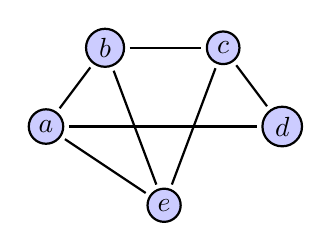
\begin{tikzpicture}[node distance=0.5cm,
                       thick,main node/.style={circle,fill=blue!20,draw,outer sep=2pt,inner sep=2pt}
                      ] 
  \node[main node] (a) at (-1.5,0) {$a$};
  \node[main node] (b) at (-0.75,1.00) {$b$};
  \node[main node] (c) at (0.75,1.00) {$c$};
  \node[main node] (d) at (1.5,0) {$d$};
  \node[main node] (e) at (0,-1.00) {$e$};
  \path%
   (a) edge [left] node {} (b)
   (a) edge [left] node {} (d)
   (a) edge [left] node {} (e)
   (b) edge [left] node {} (c)
   (b) edge [left] node {} (e)
   (c) edge [left] node {} (d)
   (c) edge [left] node {} (e);
 \end{tikzpicture}
\end{minipage}
\hspace*{0.1\textwidth}
\begin{minipage}[b]{0.4\textwidth}
 (b)\quad\linebreak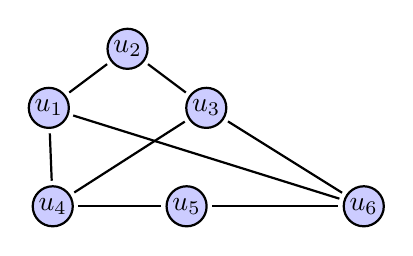
\begin{tikzpicture}[node distance=1cm,
                     thick,main node/.style={circle,fill=blue!20,draw,outer sep=2pt,inner sep=1pt}
                    ]        
   \node[main node] (u1) at (0,0) {$u_1$};
   \node[main node] (u2) at (1,0.75) {$u_2$};
   \node[main node] (u3) at (2.0,0) {$u_3$};
   \node[main node] (u5) at (1.75,-1.25) {$u_5$};
   \node[main node] (u4) at (0.05,-1.25) {$u_4$};
   \node[main node] (u6) at (4.00,-1.25) {$u_6$};       
   \path%
     (u1) edge node [right] {} (u2)  %{} is where the edge value would go
     (u2) edge [right] node {} (u3)
     (u3) edge [right] node {} (u4)
     (u4) edge [left] node {} (u1)
     (u1) edge [left] node {} (u6)
     (u4) edge [left] node {} (u5)
     (u5) edge [left] node {} (u6)
     (u3) edge [left] node {} (u6);
 \end{tikzpicture}
\end{minipage}

\underbar{Solutions} Graph (a) cannot be bipartite since it contains a triangle with the vertices $a,b,e$.\\[3pt]
Graph (b) is bipartite. It can be drawn as

\quad\linebreak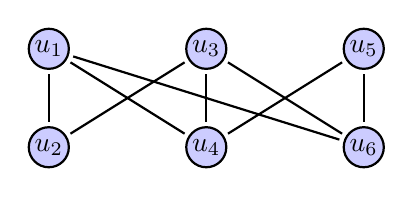
\begin{tikzpicture}[node distance=1cm,
                     thick,main node/.style={circle,fill=blue!20,draw,outer sep=2pt,inner sep=1pt}
                    ]        
   \node[main node] (u1) at (0,0) {$u_1$};
   \node[main node] (u3) at (2,0) {$u_3$};
   \node[main node] (u5) at (4,0) {$u_5$};
   \node[main node] (u2) at (0,-1.25) {$u_2$};
   \node[main node] (u4) at (2,-1.25) {$u_4$};
   \node[main node] (u6) at (4,-1.25) {$u_6$};       
   \path%
     (u1) edge node [right] {} (u2)  %{} is where the edge value would go
     (u1) edge [right] node {} (u4)
     (u1) edge [right] node {} (u6)
     (u3) edge [left] node {} (u2)
     (u3) edge [left] node {} (u4)
     (u3) edge [left] node {} (u6)
     (u5) edge [left] node {} (u4)
     (u5) edge [left] node {} (u6);
 \end{tikzpicture}\\[5pt]
 
 \item 
 For each pair of graphs either prove that $G_1\not\cong G_2$, or find a graph isomorphism $\varphi:G_1\to G_2$, and confirm $\varphi$ is
 edge-preserving using adjacency matrices.
 
\vspace*{\baselineskip}
\begin{minipage}[b]{0.4\textwidth}
(a)\quad\linebreak
    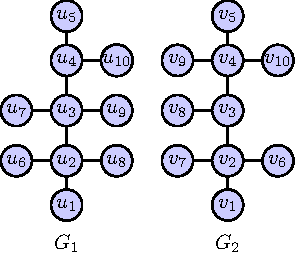
\includegraphics{./exer38-3-c.pdf}
\end{minipage}
\hspace*{0.15\textwidth}
\begin{minipage}[b]{0.4\textwidth}
 (b)\quad\linebreak
    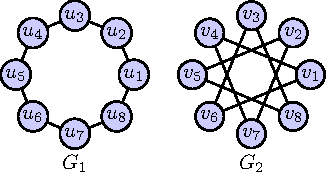
\includegraphics{./exer38-3-b.pdf}
\end{minipage}\\[5pt]

\underbar{Solutions} The graphs in (a) are not isomorphic. Notice the $G_{1}$ has two vertices, $u_{2}$ and $u_{3}$, that have degree $4$ and are adjacent. There is no such pattern in $G_{2}$, so no isomorphism is possible. The graphs in (b) are isomorphic. The easiest way to see that is to notice that we can start at $u_{1}$ in graph $G_{1}$ and travel once around the cycle in the counterclockwise direction: $u_{1}-u_{2}-u_{3}-u_{4}-u_{5}-u_{6}-u_{7}-u_{8}-u_{1}$, and we can travel a similar cycle in $G_{2}$: $v_{1}-v_{4}-v_{7}-v_{2}-v_{5}-v_{8}-v_{3}-
v_{6}-v_{1}$. That shows how to order the vertices in $G_{2}$ so the adjacency matrices will be the same for the two graphs.\\[5pt]


\item For the graph below
 \begin{enumerate}
  \item  find an Eulerian path, or prove that none exists, and 
  \item  find a Hamiltonian cycle or prove that none exists.
 \end{enumerate}
  
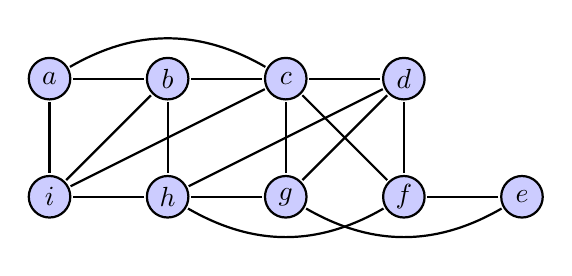
\begin{tikzpicture}[thick,main node/.style={circle,fill=blue!20,draw,outer sep=1pt,inner sep=1pt,minimum size=15pt}
                      ]  
   \node[main node] (a) at (0,1.5) {$a$};
   \node[main node] (b) at (1.5,1.5) {$b$};
   \node[main node] (c) at (3.0,1.5) {$c$};
   \node[main node] (d) at (4.5,1.5) {$d$};
   \node[main node] (i) at (0,0) {$i$};
   \node[main node] (h) at (1.5,0) {$h$};
   \node[main node] (g) at (3.0,0) {$g$};
   \node[main node] (f) at (4.5,0) {$f$};
   \node[main node] (e) at (6.0,0) {$e$};
   \path%
    (a) edge [left] node {} (b)
    (a) edge [bend left] node  {} (c)
    (a) edge [left] node {} (i)
    (b) edge [left] node {} (c)
    (b) edge [left] node {} (h)
    (b) edge [left] node {} (i)
    (c) edge [left] node {} (d)
    (c) edge [left] node {} (f)
    (c) edge [left] node {} (g)
    (c) edge [left] node {} (i)
    (d) edge [left] node {} (f)
    (d) edge [left] node {} (g)
    (d) edge [left] node {} (h)
    (e) edge [left] node {} (f)
    (e) edge [bend left] node {} (g)
    (f) edge [bend left] node {} (h)
    (g) edge [left] node {} (h)
    (h) edge [left] node {} (i);
  \end{tikzpicture}\\[3pt]
  
  \underbar{Solutions}\\[3pt]
 \begin{enumerate}
  
\item Vertices $a$ and $h$ are the only two vertices of odd degree. So there is an Eulerian path starting at $a$ and ending at $h$.\\[3pt]
  
\item A Hamiltonian cycle: $a-b-c-d-f-e-g-h-i-a.$ \\[5pt]

\end{enumerate}

\item  Answer the following questions about the rooted tree shown below.
 
 \vspace*{0.25cm}

  \begin{enumerate}
    \item Which vertex is the root?
    \item Which vertices are internal?
    \item Which vertices are leaves?
    \item Which vertices are children of $b$?
    \item Which vertices are grandchildren of $b$?
    \item Which vertex is the parent of $m$?
    \item Which vertices are siblings of $q$?
    \item Which vertices are ancestors of $p$? 
    \item  Which vertices are descendants of $d$?
    \item  What level is $i$ at?
  \end{enumerate}  



  \centering
  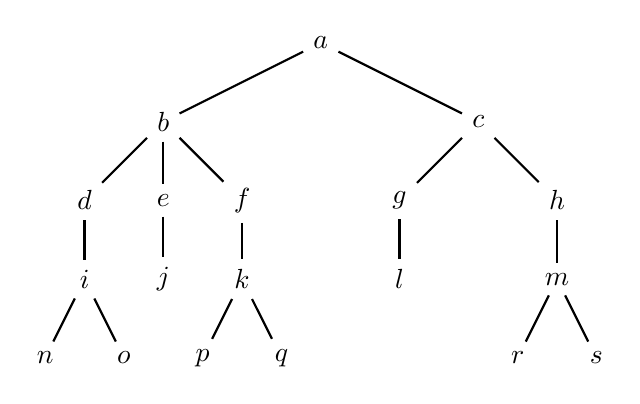
\begin{tikzpicture}[thick]
   \node (root) at (0,0) {$a$};
   \node (l) at (-2.00,-1) {$b$};
   \node (ll) at (-3.00,-2) {$d$};
   \node (llm) at (-3.00,-3) {$i$};
   \node (llml) at (-3.50,-4) {$n$};
   \node (llmr) at (-2.50,-4) {$o$};
   \node (lm) at (-2.00,-2) {$e$};
   \node (lmm) at (-2.00,-3) {$j$};
   \node (lr) at (-1.00,-2) {$f$};
   \node (lrm) at (-1.00,-3) {$k$};
   \node (lrml) at (-1.50,-4) {$p$};
   \node (lrmr) at (-0.50, -4) {$q$};
   \node (r) at (2.00,-1) {$c$};
   \node (rl) at (1.00,-2) {$g$};
   \node (rlm) at (1.00,-3) {$l$};
   \node (rr) at (3.00,-2) {$h$};
   \node (rrm) at (3.00,-3) {$m$};
   \node (rrml) at (2.50,-4) {$r$};
   \node (rrmr) at (3.50,-4) {$s$};
   \path%
     (root) edge [left] node {} (l) %a to b
     (l) edge [left] node {} (ll) %b to d
     (ll) edge [left] node {} (llm) %d to i
     (llm) edge [left] node {} (llml) %i to n
     (llm) edge [left] node {} (llmr) %i to o
     (l) edge [left] node {} (lm) %b to e
     (lm) edge [left] node {} (lmm) %e to j
     (l) edge [left] node {} (lr) %b to f
     (lr) edge [left] node {} (lrm) %f to k
     (lrm) edge [left] node {} (lrml) %k to p
     (lrm) edge [left] node {} (lrmr) %k to q
     (root) edge [left] node {} (r) %root to c
     (r) edge [left] node {} (rl) %c to g
     (rl) edge [left] node {} (rlm) %g to l
     (r) edge [left] node {} (rr) %c to h
     (rr) edge [left] node {} (rrm) %h to m
     (rrm) edge [left] node {} (rrml) %m to r
     (rrm) edge [left] node {} (rrmr); %m to s
   \end{tikzpicture}%\\[5pt]


\underbar{Solutions}
\begin{enumerate}
\item $a$
\item $b,c,d,e,f,g,h,i,k,m$
\item $j,l,n,o,p,q,r,s$
\item $d,e,f$
\item $i,j,k$
\item $h$
\item $p$ 
\item $k,f,b,a$
\item $i,n,o$
\item $3$
\end{enumerate}


\end{enumerate}

\subsection{Lesson 21: Test 3}

\begin{enumerate}

\item[]
\centerline{The third examination will cover the topics in lessons 15 through 20.}
\medskip
\centerline{\bf NO: books, notes, calculators, cell phones, scratch paper, etc}
\medskip
\centerline{\bf There is a (very generous!) $2$ hour time limit for the exam.}
\medskip

The exam is identical in format to examinations \#1 and \#2:
there are $12$ {\it True-False} questions worth $2{1\over2}$ points each, 
$8$ multiple choice questions worth $5$ points each, and $3$ {\it longer answer} 
problems worth $10$ points each. 
\medskip 

\item {\bf True \ \  False}: If $p$ is a prime, and $p\,|\,ab$, where $a$ and $b$ are integers, 
then either $p\,|\,a$ or $p\,|\,b$.

\medskip

\item The number of positive integers that divide $320$ is
\begin{enumerate}

\item $7$\\[4pt]

\item $14$\\[4pt]

\item $32$\\[4pt]

\item $160$\\[4pt]

\item $320$\\

\end{enumerate}

\medskip

\item {\bf True \ \  False}: $-123\equiv 11 \,(mod\,31)$.

\medskip

\item  Find all solutions to the congruence equation $12x\equiv 2 \,(mod\,5)$.

\medskip

\item Determine the number of {\it full house} poker hands ($5$ cards, order not important, selected
from a $52$ card deck, with $3$ cards of one rank, and $2$ cards of a second rank.)

\medskip

\item When $(2x-3y)^{25}$ is expanded, what is the coefficient of the term $x^{10}y^{15}$?

\medskip

\item How many string of length six of the $26$ letters either begin with $xx$ or end with $ooo$?

\medskip

\item {\bf True \ \  False}: For any finite sets $A$ and $B$, $|A\cup B| = |A| + |B|$.

\medskip

\item Find a closed form formula for $a_0 = 1$, $a_1 = 1$, and for $n\geq2$, $a_n = 3a_{n-1} + 10a_{n-2}$.

\medskip

\item {\bf True \ \  False}: When solving a nonhomogeneous recursion with recursive relation
$a_n = 2a_{n-1} + n^2 + 1$, a good choice for the form of a particular solution is $a_n^{(p)} =  An^2 + 1$.

\medskip
 
 \item {\bf True \ \  False}: Every graph with a Eulerian path will have an Eulerian cycle.
 
 \medskip

\item {\bf True \ \  False}: Every tree with $10$ vertices must have $9$ edges. 

\medskip

\item {\bf True \ \  False}: The wheel, $W_{10}$, has a Hamiltonian cycle.

\end{enumerate}

\vskip 20pt


\begin{center}
Hints and Solutions to Sample Questions
\end{center}

\medskip

\begin{enumerate}

\item True. This is one of the basic properties we proved for primes.

\medskip

\item Since $320 = 32\cdot 10 = 64\cdot 5 = 2^6\cdot 5$, we know positive divisors will look
like $2^a\cdot5^b$ where $a$ can be any of the seven values $0,1,2,3,4,5,6$ while $b$ has two
options: $0,1$. That gives a grand total of $7\cdot2 = 14$ positive integers that divide $320$.

\medskip

\item False since $11-(-123) = 134$ is not divisible by $31$. 

\medskip

\item Since $12\equiv 2\,(mod\,5)$, the stated problem is the same as $2x\equiv 2\,(mod\,5)$,
and since obviously $x\equiv 1\,(mod\,5)$ is the only solution to that equivalence equation.

\medskip

\item Answer: $\displaystyle \binom{13}{1}\binom{4}{3}\binom{12}{1}\binom{4}{2}$. Reasoning: we first pick one
of the thirteen ranks for the three of a kind, then pick three of the four cards of that rank, then pick one of the twelve remaining ranks for the pair, then two of the four cards of that rank. Since we need to do all four tasks, we use the product rule. 


\medskip


\item The term involving $x^{10}y^{15}$ is $\displaystyle \binom{25}{10}(2x)^{10}(-3y)^{15}$, and so the
coefficient is $\displaystyle -\binom{25}{10}2^{10}3^{15}$. We'll leave the answer in this form of course!


\medskip

\item Let's use inclusion-exclusion to do the counting. Let $X$ be the set of strings that begin $xx$, 
and $O$ the set of strings that end $ooo$. We need to count $X\cup O$.

\[
|X\cup O| = |X| + |O| - |X\cap O| = 26^4 + 26^3 - 26
\]

\medskip

\item False. The stated relation is correct only if $A$ and $B$ are disjoint.

\medskip

\item The characteristic equation is $r^2 -3r-10 = 0$. The left side factors as $(r+2)(r-5)$, so the characteristic
roots are $r = -2, 5$. That means the general solution is $a_n = A(-2)^n + B(5^n)$.

The initial conditions require  $1 = A + B$  and $1 = -2A + 5B$. Multiplying the first equation by $2$ and adding
it to the second shows $3 = 7B$ so $\displaystyle B = \frac{3}{7}$. Since $A+B=1$, we must have 
$\displaystyle A= \frac{4}{7}$.
So the solution is $\displaystyle a_n = \left(\frac{4}{7}\right)(-2)^n + \left(\frac{3}{7}\right)5^n$. 

\medskip

\item False. The correct form of the guess is the most general form of the nonhomogeneous part, and that would be
$An^2+Bn+C$.

\medskip

\item False. Example: The $3$-link, $L_{3}$ has a Eulerian path, but does not have a Eulerian cycle.

\medskip 

\item True. The number of edges in a tree is always one less than the number of vertices.
 
\medskip

\item True. Start at the {\it axle} vertex, go out to the {\it rim}, to a vertex $a$, go around the rim
(say clockwise, just to be specific) until you reach the vertex {\it just one before} $a$, and then return
to the axle vertex.


\end{enumerate}


\end{document}